\documentclass[11pt]{article}

\usepackage[margin=1.1in]{geometry}
\usepackage{amsmath, amssymb, amsthm}
\usepackage{booktabs}
\usepackage{array}
\newcolumntype{L}[1]{>{\raggedright\arraybackslash}p{#1}}
\usepackage{enumitem}
\usepackage{xcolor}
\usepackage{graphicx}
\usepackage{float}
\usepackage{comment}
\graphicspath{{figures/}}
\usepackage[colorlinks=true, linkcolor=blue!60!black, urlcolor=blue!60!black]{hyperref}

%% Line numbers for review - comment out this block to remove them.
\usepackage[mathlines]{lineno}
\renewcommand{\linenumberfont}{\normalfont\tiny\sffamily\color{gray}}
% number the lines of amsmath display environments too
\newcommand*\patchAmsMathEnvironmentForLineno[1]{%
\expandafter\let\csname old#1\expandafter\endcsname\csname #1\endcsname \expandafter\let\csname oldend#1\expandafter\endcsname\csname end#1\endcsname
  \renewenvironment{#1}%
     {\linenomath\csname old#1\endcsname}%
     {\csname oldend#1\endcsname\endlinenomath}}%
\newcommand*\patchBothAmsMathEnvironmentsForLineno[1]{%
  \patchAmsMathEnvironmentForLineno{#1}%
  \patchAmsMathEnvironmentForLineno{#1*}}%
\AtBeginDocument{%
  \patchBothAmsMathEnvironmentsForLineno{equation}%
  \patchBothAmsMathEnvironmentsForLineno{align}%
  \patchBothAmsMathEnvironmentsForLineno{gather}%
  \patchBothAmsMathEnvironmentsForLineno{multline}%
}
\linenumbers

\setlist[itemize]{itemsep=2pt, topsep=3pt, parsep=0pt, leftmargin=1.4em}
\newtheorem{proposition}{Proposition}
\newtheorem{result}{Result}
\newtheorem{lemma}{Lemma}
\theoremstyle{remark}
\newtheorem{remark}{Remark}

\newcommand{\jnote}[1]{\textcolor{gray}{\textit{[#1]}}}
\newcommand{\flag}[1]{\textcolor{red!70!black}{[\textbf{Flag:} \textit{#1}]}}
\newcommand{\E}{\mathbb{E}}
\newcommand{\Var}{\mathrm{Var}}
\newcommand{\Cov}{\mathrm{Cov}}
\newcommand{\Corr}{\mathrm{Corr}}

\title{Conceptual framework and identification}
%\date{}

\begin{document}
\maketitle

%
%\subsection*{Changes relative to v4}
%\begin{itemize}
%\item The case ladder is now: Case 1 (i.i.d., stationary variance), Case 2 (AR(1), stationary variance), Case 3 (AR(1), age-specific variances). Case 3 was the appendix general case.
%\item The proposition reads each case off two curves - the variance profile $V(a)$ and the first row $C_0(a)$ - plus, in Case 3, two cells from the interior of the matrix.
%\item New Result 6: the value of targeting on initial health, with a gap channel and a compounding channel.
%\item New figures: one two-panel chart per case; $K(r)$ assembled from identified blocks.
%\item New Section 3.3: the forces behind identification, one region of the matrix at a time.
%\item Appendix F keeps the general template, the denoising case and the random-walk proposition.
%\end{itemize}

%% =============================================================================
\section{Framework}
%% =============================================================================

\subsection{Health process}

\begin{itemize}
\item Health of individual $i$ of (latent) type $j$ at age $a\in\{0,1,\dots,\bar a\}$ is the type's mean path plus an individual shock:
\begin{equation}
h_{i,a} \;=\; \bar h_{j,a} + u_{i,a},
\qquad
\bar h_{j,a} \;\equiv\; H_j + \sum_{a'=1}^{a} d_{j,a'},
\label{eq:levels}
\end{equation}
\item Age $a$ counts from a \emph{base age} - the start of the window being modelled - not from birth: $a=0$ is the base age and $\bar a$ the end of the horizon.
\item $\{H_j,(d_{j,a})_a\}$ is the \emph{deterministic} component: $H_j$ the type's level at the base age (so $\bar h_{j,0}=H_j$), $d_{j,a}$ its expected health change at age $a$.
$H_j$ is the accumulated outcome of everything before the window - early conditions, past decline, shocks that have landed - and nothing below requires the base age to be birth.
\item Types need not be coarse groups: in the limit each individual is their own type, which is the continuous case of Section~\ref{sec:linear}, where every person has their own $(H_i,d_i)$.
\item $u_{i,a}$ is the \emph{stochastic} component: $\E[u_{i,a}\mid j]=0$ at every age, but otherwise we are agnostic as to its distribution.
\item At the base age: $h_{i,0}=H_j+u_{i,0}$
\end{itemize}

\subsection{What stays, what is in the moment, what evolves}\label{sec:triad}

\begin{itemize}
\item A useful reading of \eqref{eq:levels}: at any age, a health history carries three kinds of information -
  \begin{itemize}
\item what \emph{stays} with you: your current level - the type intercept plus anything permanent that has already landed;
\item what is \emph{in the moment}: transitory variation and measurement error, gone by the next wave;
\item how you are \emph{evolving}: the deterministic drift $d_{j,a}$ - the only component that predicts future \emph{changes}.
  \end{itemize}
\item Prevention targets the third; treatment acts on the first two as realized (the gap, however it arose).
\item Note that a permanent shock, once landed, belongs to ``stays'': that is why levels bundle it with the type intercept (Section~\ref{sec:ident}), and why the returns will not care about that split.
\item Partly persistent shocks sit between ``stays'' and ``in the moment'': a shock is carried forward in proportion to its memory, which is what Section~\ref{sec:forces} reads off the data.
\item Only what is carried from one wave to the next can produce covariance between waves.
This single fact drives all of Section~\ref{sec:ident}: the three components leave different traces on the covariance matrix, and identification is reading them apart (Section~\ref{sec:forces}).
\end{itemize}

\subsection{Deterministic versus stochastic and targeted prevention}\label{sec:detstoch}

Prevention acts on the deterministic dynamic process (the dynamics $d_{j,a}$); treatment acts on the realized distribution of $h$.
\\~\\
To target prevention one must predict. Predictability is necessary for targetability but not sufficient. Classifying by the source of the dispersion in health, and by whether policy can act on it:

\begin{center}
\begin{tabular}{@{}lll@{}}
	\toprule
	\textbf{Dispersion is} & \textbf{Actionable} & \textbf{Not actionable} \\
	\midrule
	deterministic (across types) & targetable prevention & limits of medical science \\
	stochastic (within type) & untargeted prevention; treatment & pure noise \\
	\bottomrule
\end{tabular}
\end{center}

\noindent Reading the four cells:
\begin{itemize}
\item Deterministic and actionable: decline differs predictably across types, so prevention can be aimed at the types with most to gain.
\item Deterministic and not actionable: the decline is predictable but nothing can be done about it.
\item Stochastic and actionable: prevention still works, because everyone shares the same mean dynamics; what dies is \emph{targeting}, not prevention.
Treatment also sits here, since it acts on realized health whatever produced it.
\item Stochastic and not actionable: unpredictable and untreatable variation.
\end{itemize}

\noindent Other points to note:
\begin{itemize}
\item Permanent vs.\ transitory is secondary: persistence scales the value of prevention or treatment, but whether it can be targeted depends on whether it is deterministic vs.\ stochastic.
\item Predictability of levels $\neq$ predictability of changes: persistent stochastic realizations predict future levels, but only the deterministic component predicts future changes (and prevention targets changes).
\item Types don't need to be literally deterministic: $d_{j,a}$ is the type-conditional expected change (e.g.\ a type-specific hazard $\times$ shock severity in a life-course model).
Prevention targets the conditional mean; within-type persistent shocks are treatable but not ex-ante targetable.
\item While we can imagine interventions that change the variance without the mean (e.g. deregulating the drug market), these are secondary to interventions that shift the mean.
\end{itemize}

\begin{figure}[H]
	\centering
	\caption{Gain from targeting prevention on dynamics is large in (a) and zero in (b)}
	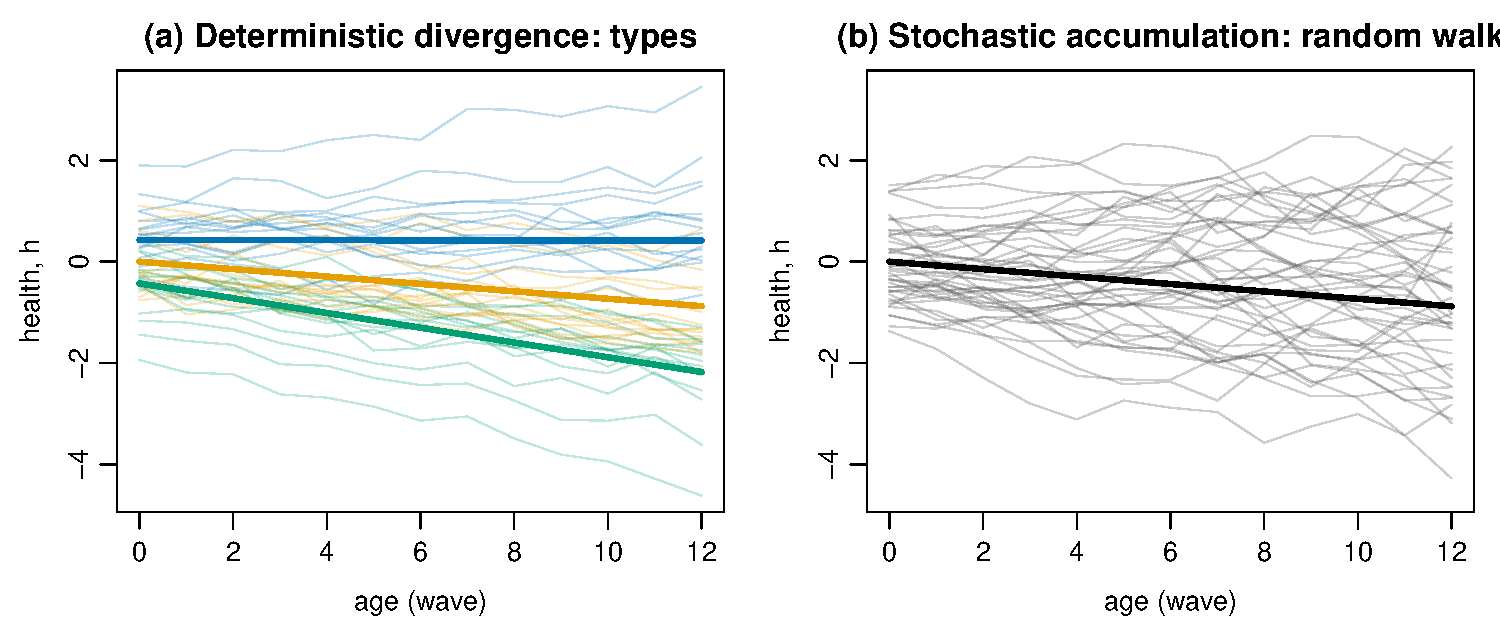
\includegraphics[width=\textwidth]{fig_two_worlds.pdf}
	\label{fig:twoworlds}
\end{figure}
\vspace*{-0.6cm} Figure~\ref{fig:twoworlds} visualises the deterministic vs stochastic distinction: two simulated populations with the same cross-sectional health distribution (so healthcare cost is the same at every age).
In panel (a) the dispersion comes from continuously distributed types $(H_i,d_i)$, so future decline differs predictably and targeting has value.
In panel (b) it comes from a random walk, so expected future decline is the same for everyone and there is no role for targeted prevention.
To work out which world we are in, we need dynamic moments.


\subsection{Connection to types}

Types are the object of interest because they are what makes targeted prevention possible: if decline differs predictably across groups, intensity can be aimed at the groups with most to gain - the actionable column of Section~\ref{sec:detstoch}.

\begin{itemize}
\item Types represent the distribution of the deterministic components $(H,d)$, and clustering can estimate this.
The deterministic/stochastic split maps to between vs.\ within variance, and to type vs.\ individual.
\item Individuals who sit persistently above or below their type indicate that we have identified too few types: deterministic heterogeneity is leaking into the within component.
\item Individuals fluctuating around their type mean, by contrast, are showing the stochastic component $u$.
\item With the base age at birth, the three standard life-course accounts map one-to-one to the framework's second moments: \emph{critical-period} models (early conditions leave a lasting level effect) are $\Var(H)$; \emph{accumulation} models (disadvantage builds up through the rate of decline) are $\Var(d)$; \emph{pathway} models (early disadvantage shapes the later rate) are $\Cov(H,d)$.
\item At a later base age, $\Var(H)$ is the accumulated outcome of all three.
The accounts are then separated not by one number but by how the triple $(\Var(H),\Cov(H,d),\Var(d))$ evolves as the base age moves - which is what the data section estimates.
Section~\ref{sec:ident} identifies the triple at a given base age.
\end{itemize}

%% =============================================================================
\section{Healthcare costs and the two instruments}\label{sec:cost}
%% =============================================================================

\subsection{Cost of poor health}

\begin{itemize}
\item Cost of health: $c(h)=(1-h)^2$, with the maximum level of health normalised to one.
\item The quadratic is the second-order approximation to any smooth increasing convex cost, and it is what makes the first two moments of health sufficient for the policy objects below.
\item Convexity is in the data: healthcare use is convex in $h$ on every metric, with quadratic terms carrying $t$-statistics of 15 to 40 (Figure~\ref{fig:convexdata}).
It is mildest on the primary measure, whose cardinalisation spreads the sick finely, and strongest on the utility-weighted SF-6D - the closest thing to cost we observe.
\end{itemize}

\begin{figure}[H]
	\caption{In-patient admission probability against health, in equal-width bins of each measure's own units, with the fitted quadratic. Convex on both metrics: mildly on the primary measure (quadratic $t=15$), strongly on the utility-weighted SF-6D ($t=40$).}
	\label{fig:convexdata}
	\centering
	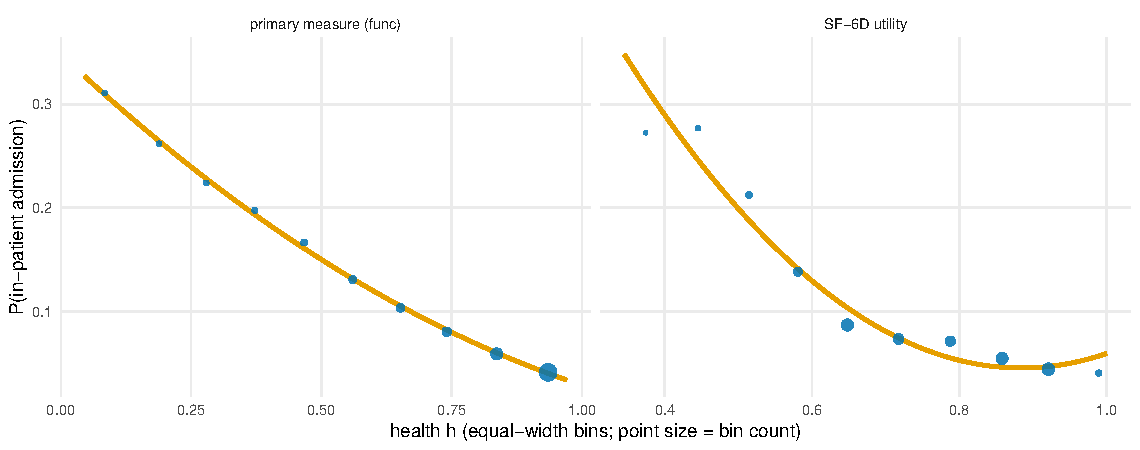
\includegraphics[width = 0.8 \linewidth]{emp_fig_v6_convexity}
\end{figure}

\begin{itemize}
\item Type-level expected cost at age $a$:
\begin{equation}
\E\left[c(h_{i,a})\mid j\right] \;=\; \bigl(1-\bar h_{j,a}\bigr)^2 + \Var(u_{i,a}\mid j).
\end{equation}
\item Population expected cost at age $a$ (shares $\pi_j$, population mean health $\bar h_a=\sum_j\pi_j \bar h_{j,a}$):
\begin{equation}
\E\left[c(h_{i,a})\right]
\;=\;
\underbrace{\bigl(1-\bar h_a\bigr)^2}_{\text{mean gap}}
\;+\;
\underbrace{\textstyle\sum_j \pi_j\bigl(\bar h_{j,a}-\bar h_a\bigr)^2}_{\text{between types}}
\;+\;
\underbrace{\textstyle\sum_j \pi_j\,\Var(u_{i,a}\mid j)}_{\text{within types}} .
\label{eq:popcost}
\end{equation}
\item Lifetime cost of individual $i$: $\mathcal{C}_i\equiv\sum_{a=0}^{\bar a}c(h_{i,a})$.
\item Notation: moments subscripted by $j$ ($\E_j$, $\Var_j$, $\Cov_j$, $\mathrm{sd}_j$) are taken across types with weights $\pi_j$; unsubscripted moments are across individuals.
For type-level objects the two coincide (an individual inherits their type's value); the distinction matters for health itself, where $\Var_j(\bar h_{j,a})$ is the between-type term in \eqref{eq:popcost} while $\Var(h_{i,a})$ is the total variance.
If each individual is their own type, the between-type term collects all deterministic dispersion and the within-type term is pure noise, $\Var(u_{i,a})$.
\end{itemize}

\subsection{A linear case}\label{sec:linear}

\begin{itemize}
\item For intuition, and for identification later, take the type mean changes to be constant, $d_{j,a}=d_j$. Then
\begin{equation}
h_{i,a}=H_i+a\,d_i+u_{i,a}, \qquad a=0,1,2,\dots
\label{eq:linwindow}
\end{equation}
a random-coefficients growth model: individual intercepts and slopes $(H_i,d_i)$, with types as their discrete support.
\item Parameters: $V_H\equiv\Var(H_i)$, $V_d\equiv\Var(d_i)$, $C_{Hd}\equiv\Cov(H_i,d_i)$, $v_a\equiv\Var(u_{i,a})$ (written $\sigma^2_u$ when it does not vary with age).
Sign: $C_{Hd}>0$ $\Leftrightarrow$ types worse off at the base age decline faster; $C_{Hd}<0$ $\Leftrightarrow$ catching up.
\item The parameters map to observed moments as (with $\bar H\equiv\E[H_i]$, $\bar d\equiv\E[d_i]$)
\begin{equation}
	\begin{gathered}
		\bar h_a=\bar H+a\,\bar d, \qquad
		\Var(h_a)=V_H+2aC_{Hd}+a^2V_d+v_a, \\\
		\Cov(h_s,h_t)=V_H+(s+t)C_{Hd}+st\,V_d+\Cov(u_s,u_t).
	\end{gathered}
\label{eq:forwardmap}
\end{equation}
\item Section~\ref{sec:ident} shows how we can invert this map: the parameters $(V_H,C_{Hd},V_d)$ and the noise are recovered from observed moments.
\item The linear case carries the intuition and is what Section~\ref{sec:ident} identifies.
In the data, decline is not straight over long spans, and we add a quadratic age term; that is a larger deterministic basis in the general template of Appendix~\ref{app:surface} ($f=\{1,a,a^2\}$), not a different framework - it costs extra parameters and hence extra waves.
\end{itemize}

\subsection{Treatment: ex post, on realizations}

\begin{itemize}
\item Treatment is an ex-post proportional reduction of the realized gap $h\mapsto h+\tau(1-h)$, so each age-$a\ge r$ cost term scales by $(1-\tau)^2$.
\end{itemize}

\begin{result}[Return to treatment]\label{res:treat}
The marginal return to treatment beginning at age $r$ is
\begin{equation}
T(r) \;\equiv\; -\,\tfrac{\partial\,\E[\mathcal{C}_i(\tau;r)]}{\partial\tau}\Big|_{\tau=0}
\;=\; 2\sum_{a=r}^{\bar a}\E\bigl[(1-h_{i,a})^2\bigr]
\;=\; 2\sum_{a=r}^{\bar a}\Bigl[\bigl(1-\bar h_a\bigr)^2+\Var(h_{i,a})\Bigr].
\end{equation}
\end{result}

\begin{itemize}
\item The factor of $2$ is the derivative of the square: scaling the gap by $(1-\tau)$ makes the age-$a$ cost $(1-\tau)^2(1-h_{i,a})^2$.
It appears in every return for the same reason, so it cancels in every comparison below.
\item Treatment leaves the underlying process untouched: it rescales the realized gap at each age, and does not change the health an individual brings into the next age.
\item Read plainly, $T(r)$ is twice the expected cost still to come from age $r$ onwards.
\item Treatment works through the total variance - between \emph{and} within, including the stochastic component.
\item $T(r)$ thus requires only cross-sectional moments: the treatment/healthcare-cost side of the framework is directly observable (no identification problem).
\end{itemize}

\jnote{A potential extension for the counterfactuals we could highlight here - discount future ages by survival, $\sum_{a\ge r}S(a\mid r)(\cdot)$.
Works two ways: prevention less valuable as the sickest will die, but prevention could raise survival chances.}

\subsection{Prevention: ex ante, on deterministic dynamics}\label{sec:prevention}

\begin{itemize}
\item Prevention of intensity $\mu$ from age $r$ onwards works through the deterministic change:
\begin{equation}
\Delta h_{i,a}(\mu) = (1-\mu)\,d_{j,a} + \Delta u_{i,a} \quad (a\ge r)
\qquad\Longrightarrow\qquad
h_{i,a}(\mu) = h_{i,a} + \mu\,\bigl(\bar h_{j,r-1}-\bar h_{j,a}\bigr),
\end{equation}
since $-\mu\sum_{a'=r}^{a}d_{j,a'}=\mu(\bar h_{j,r-1}-\bar h_{j,a})$: the health gained is $\mu$ times the type's \emph{preventable decline}, the mean health lost between the pre-intervention age $r-1$ and age $a$ ($>0$ for declining types).
The first change scaled is the one from $r-1$ into $r$, so prevention takes a share $\mu$ of the deficit that would open during year $r$: think of it as an intervention at the start of year $r$, after $h_{i,r-1}$ is observed.
\item Unlike treatment, prevention compounds: it scales down every future change, so the health it saves accumulates over the remaining horizon.
\item Uniform prevention can be thought of as ``slowing ageing'': every type's rate of change is scaled by $(1-\mu)$, so trajectories stretch out in age, while treatment repairs the gaps that ageing has already produced.
\item Prevention shifts means only here. We could of course allow interventions on the variance by letting $\mu$ also scale $\Var(u_{i,a}\mid j)$ in \eqref{eq:popcost}, but that's an extension.
\end{itemize}

\jnote{An alternative set up could be flagged here and tried in the counterfactuals - instead of scaling $d_j$, let prevention move a person to a better type, so the return is the gap between two type paths rather than a derivative along one.}

\begin{result}[Return to prevention, type/individual level]\label{res:prevj}
\begin{equation}
P_j(r) \;\equiv\; -\,\tfrac{\partial\,\E[\mathcal{C}_i(\mu;r)\mid j]}{\partial\mu}\Big|_{\mu=0}
\;=\; 2\sum_{a=r}^{\bar a} \bigl(1-\bar h_{j,a}\bigr)\bigl(\bar h_{j,r-1}-\bar h_{j,a}\bigr).
\end{equation}
\end{result}

\begin{itemize}
\item Value $=$ gap $\times$ preventable decline, summed over remaining life, so large when the type is \emph{already} far from full health and has a lot of decline coming up.
\item Sign convention: the returns are the \emph{signed} negative derivatives.
$T(r)$ is always positive; $P_j(r)$ is positive for net-declining types and negative for improving ones (for whom scaling the dynamics down means scaling improvement down).
The signed form is what aggregates exactly in Result~\ref{res:prevpop}.
\end{itemize}

\begin{result}[Return to \emph{uniform} prevention, population level]\label{res:prevpop}
For a uniform policy - the same $\mu$ applied to everyone,
\begin{equation}
P(r) \;=\; \sum_j \pi_j P_j(r)
\;=\; 2\sum_{a=r}^{\bar a}\Bigl[\bigl(1-\bar h_a\bigr)\bigl(\bar h_{r-1}-\bar h_a\bigr)
\;+\; \Cov_j\bigl(1-\bar h_{j,a},\,\bar h_{j,r-1}-\bar h_{j,a}\bigr)\Bigr].
\label{eq:Ppop}
\end{equation}
\end{result}

\begin{itemize}
\item The mean channel pairs the population gap with the population's own mean decline - both directly observable.
\item Even though there is no targeting here, the between-type covariance appears anyway because the intervention is multiplicative in the type's own decline $d_{j,a}$, so types with more decline get more from the same $\mu$.
\item The covariance is positive when lower-health types are also those with more preventable decline; prevention then compresses trajectories.
\item In level-covariance terms the channel is $\Var_j(\bar h_{j,a})-\Cov_j(\bar h_{j,a},\bar h_{j,r-1})$: how far types have fanned out by age $a$, over and above the spread they already had when the policy started.
If types kept the same spacing after $r-1$ the two terms would be equal and the channel would vanish.
\item Those two moments are the diagonal cell at $a$ and the $(r-1,a)$ cell of the covariance matrix, with the noise stripped out.
This already introduces our framework that prevention returns are priced by particular cells of the covariance surface, and Section~\ref{sec:ident} is about recovering them.
\item The gain from \emph{deliberately} targeting (choosing $\mu_j$ by type) is measured against this uniform benchmark in Result~\ref{res:type}.
\item Decomposition of the between-type channel: split the health gap into initial gap, pre-intervention decline, and preventable decline, $1-\bar h_{j,a}=(1-H_j)+(H_j-\bar h_{j,r-1})+(\bar h_{j,r-1}-\bar h_{j,a})$.
Then:
\begin{equation}
	\begin{gathered}
		\Cov_j\bigl(1-\bar h_{j,a},\,\bar h_{j,r-1}-\bar h_{j,a}\bigr)
		= \\
		\underbrace{\Cov_j\bigl(1-H_j,\,\bar h_{j,r-1}-\bar h_{j,a}\bigr)}_{\text{initial disadvantage}\times\text{later decline}}
		+
		\underbrace{\Cov_j\bigl(H_j-\bar h_{j,r-1},\,\bar h_{j,r-1}-\bar h_{j,a}\bigr)}_{\text{persistence of decline}}
		+
		\underbrace{\Var_j\bigl(\bar h_{j,r-1}-\bar h_{j,a}\bigr)}_{\text{dispersion of decline}} .
	\end{gathered}
\label{eq:covdecomp}
\end{equation}
The three channels are the pathway margin (initial disadvantage $\times$ later decline), the persistence margin, and the dispersion-of-decline (accumulation) margin; each maps to moments identified in Section~\ref{sec:ident}.
\end{itemize}

\subsection{Comparing the two instruments}\label{sec:compare}

\begin{result}[Prevention vs.\ treatment]\label{res:T3}
Compare compositions:
\begin{align}
T(r) &= 2\sum_{a\ge r}\Bigl[(1-\bar h_a)^2 + \underbrace{\Var_j\bigl(\bar h_{j,a}\bigr)}_{\text{between}}
+ \underbrace{\textstyle\sum_j\pi_j\Var(u_{i,a}\mid j)}_{\text{within}}\Bigr], \\
P(r) &= 2\sum_{a\ge r}\Bigl[(1-\bar h_a)\bigl(\bar h_{r-1}-\bar h_a\bigr) + \Cov_j\bigl(1-\bar h_{j,a},\,\bar h_{j,r-1}-\bar h_{j,a}\bigr)\Bigr].
\end{align}
Treatment reaches all realized dispersion, including the stochastic within-type part, but only scales down gaps that have already opened.
Prevention averts future gaps but must be assigned ex ante on predictions.
A uniform policy pays the population-average preventable decline $\bar h_{r-1}-\bar h_a$: intensity goes to slow decliners and improvers as well as to steep decliners, and the same total intensity concentrated on the steep decliners would buy more.
Its between-type channel is bounded by deterministic heterogeneity.
\end{result}

\begin{itemize}
\item Both returns are per-person objects: they are derivatives of the expected lifetime cost of a randomly drawn individual, so an economy-wide total is $N$ times either one and no comparison here depends on population size.
\item A caveat on the treatment side: if part of measured variance is measurement error rather than genuine health variation, it should be excluded from $\Var(h_a)$ in $T(r)$ - the only decomposition treatment ever needs.
Measurement error appears as a diagonal spike, a term that lives only on the variances (Appendix~\ref{app:surface}); the prevention return never contains it.
Case 4 of Section~\ref{sec:cases} separates the spike from genuine transitory health, which is what makes the exclusion operational.
\item The value of deliberately targeting prevention is a per-person statement in a different sense: returns differ across people, so it matters where a unit of intensity goes.
Section~\ref{sec:target0} prices this - what any allocation collects (Result~\ref{res:collect}), what initial health collects (Result~\ref{res:target}), and the ceiling set by the type itself (Result~\ref{res:type}).
\item Derivations for this section are in Appendix~\ref{app:derivations}.
\end{itemize}

\subsection{Targeting}\label{sec:target0}

Prevention must be assigned before outcomes are seen, so the question is not only how much intensity to use but where it goes.
This subsection asks what targeting is worth: first as an identity that holds for any signal, then for the simplest feasible signal (initial health), then for the best possible signal (the type itself).

\begin{result}[What targeting collects]\label{res:collect}
Let $\mu(z)$ be any allocation of prevention intensity based on information $z$, holding average intensity fixed. The saving over the uniform policy is
\begin{equation}
\Cov\bigl(\mu(z),\,\E[P_i\mid z]\bigr).
\label{eq:collect}
\end{equation}
Moving one unit of intensity from a person with signal $z'$ to a person with signal $z$ saves $\E[P_i\mid z]-\E[P_i\mid z']$.
\end{result}

\begin{itemize}
\item Targeting is worth exactly the covariance between where intensity goes and what it buys there.
\item It is zero when predicted returns do not vary with $z$: a signal that does not separate people is worth nothing, however well it predicts health.
\item The per-person form is the practical one - what matters is the difference in predicted returns between the person treated and the person not treated.
\item The value of a signal is therefore how much predicted returns differ across people who differ in it. The rest of this subsection computes that for two signals.
\item Per unit of dispersion in intensity, no rule based on $z$ can save more than $\mathrm{sd}\bigl(\E[P_i\mid z]\bigr)$ (Appendix~\ref{sec:targeting}).
\end{itemize}

\begin{result}[Targeting on initial health]\label{res:target}
Let the signal be initial health $h_{i,0}$ - the level at the base age. Since $P_i$ depends on the individual only through their type,
\begin{equation}
\Cov\bigl(h_{i,0},P_i(r)\bigr)=\Cov_j\bigl(\bar h_{j,0},P_j(r)\bigr),
\end{equation}
and the linear projection of $P_i(r)$ on $h_{i,0}$ has slope
\begin{equation}
\beta(r)=\frac{\Cov\bigl(h_{i,0},P_i(r)\bigr)}{\Var_j(\bar h_{j,0})+v_0}.
\label{eq:beta0}
\end{equation}
If the type mean paths have zero third central moments (for example jointly normal type parameters), the covariance splits by age into two channels:
\begin{equation}
\Cov\bigl(h_{i,0},P_i(r)\bigr)=2\sum_{a\ge r}\Bigl[
\underbrace{-\bigl(\bar h_{r-1}-\bar h_a\bigr)\Cov_j\bigl(\bar h_{j,0},\bar h_{j,a}\bigr)}_{\text{gap channel}}
+\underbrace{\bigl(1-\bar h_a\bigr)\Cov_j\bigl(\bar h_{j,0},\,\bar h_{j,r-1}-\bar h_{j,a}\bigr)}_{\text{compounding channel}}\Bigr].
\label{eq:G0}
\end{equation}
\end{result}

In the linear case $\Cov_j(\bar h_{j,0},\bar h_{j,a})=V_H+aC_{Hd}$, and the preventable decline is exposure time $(a-r+1)$ times the type's own slope, so
\begin{equation}
\Cov\bigl(h_{i,0},P_i(r)\bigr)
=2\sum_{a\ge r}(a-r+1)\Bigl[\bar d\bigl(V_H+aC_{Hd}\bigr)+C_{Hd}\bigl(\bar H-1+a\bar d\bigr)\Bigr],
\label{eq:G0lin}
\end{equation}
the first term inside the bracket being the gap channel and the second the compounding channel.

\begin{itemize}
\item The expected return falls by $|\beta(r)|$ per unit of initial health.
\item The gap channel is the mean preventable decline times how strongly initial health predicts \emph{future levels}: low initial health predicts a larger future gap, and a given decline is worth more to prevent when the gap is large.
\item The compounding channel is the mean gap times how strongly initial health predicts the \emph{decline itself}.
It is zero exactly when initial health does not predict subsequent decline; the gap channel survives even then.
\item Under decline and compounding ($\bar d<0$, $\bar H<1$, $C_{Hd}\ge0$) both channels are negative, so $\beta(r)<0$: lower $h_0$ means a higher expected return.
\item Both inputs are cells of the first row of the covariance matrix with the noise removed - $\Cov_j(\bar h_{j,0},\bar h_{j,a})$, and its difference from $\Cov_j(\bar h_{j,0},\bar h_{j,r-1})$.
Targeting on initial health is priced by the first row and the mean path.
%\item Per-person comparisons follow from the projection. A person one standard deviation below average initial health has predicted return $|\beta(r)|\,\mathrm{sd}(h_0)$ above the population mean; moving one unit of intensity from a person one sd above to one one sd below saves $2|\beta(r)|\,\mathrm{sd}(h_0)$, with average intensity unchanged.
\item $h_0$ is a noisy signal of the type's level: the slope is attenuated by $\lambda_0=\Var_j(\bar h_{j,0})/\bigl(\Var_j(\bar h_{j,0})+v_0\bigr)$ relative to observing that level, and the per-sd comparison by $\sqrt{\lambda_0}$.
Targeting benefits from the level/noise split.
\item Every input is identified in Section~\ref{sec:ident}.
\item The same logic at $z=h_{i,r-1}$ is Result~\ref{res:T2} in Appendix~\ref{sec:targeting}.
\item Proof in Appendix~\ref{sec:targeting}.
\end{itemize}

\begin{result}[Type targeting, and the ceiling]\label{res:type}
With the type as the signal, moving one unit of intensity from type $j'$ to type $j$ saves $P_j(r)-P_{j'}(r)$, and treating the highest-return type rather than a random person saves
\begin{equation}
\max_j P_j(r)-\sum_j\pi_jP_j(r).
\end{equation}
No signal does better: since $P_i$ depends on the individual only through their type, any other signal predicts returns only through what it reveals about the type, so $\Var\bigl(\E[P_i\mid z]\bigr)\le\Var_j\bigl(P_j(r)\bigr)$ for every $z$.
\end{result}

\begin{itemize}
\item The type is the ceiling because it is the whole of what determines the return; every other signal is a coarser view of it.
\item The gap between what initial health collects (Result~\ref{res:target}) and this ceiling is what estimating types is worth.
%\item These gains are not second-moment objects: $P_j(r)$ is quadratic in the type parameters, so its spread across types involves third and fourth moments of the type distribution - beyond the covariance surface of Section~\ref{sec:ident}, and the formal job of clustering.
% \item Two forces keep any level signal below the ceiling: a single level reveals only one combination of the traits that drive the return, and noise in that level attenuates it. Appendix~\ref{sec:targeting} gives the ratio and factorizes it into the two.
\end{itemize}

%% =============================================================================
\section{Identification}\label{sec:ident}
%% =============================================================================

The treatment/healthcare side (Result~\ref{res:treat}) needs only cross-sectional $\Var(h_a)$.
The prevention side (Results~\ref{res:prevj}-\ref{res:T3}) needs the between-type moments, which are not directly observable.

Figure~\ref{fig:threepanel} shows the raw material: the primary measure's mean path, its variance profile, and the rows of its covariance matrix.
Three patterns stand out before any model.
The mean falls in an accelerating way.
The variance rises steeply and then, from about age 60, stops growing.
And every row drops sharply in its first year - health not carried even one year - after which the young rows run flat while the old rows keep falling.
The rest of the section builds the machinery that reads these patterns, and the close of the section returns to them.

\begin{figure}[H]
	\caption{The primary measure over the life course: the mean path, the variance profile, and the rows of the covariance matrix. The variance and covariance panels share a vertical scale, so the drop from the profile to each row leaving it is the one-year spike. Profiles are five-year centred rolling means.}
	\label{fig:threepanel}
	\centering
	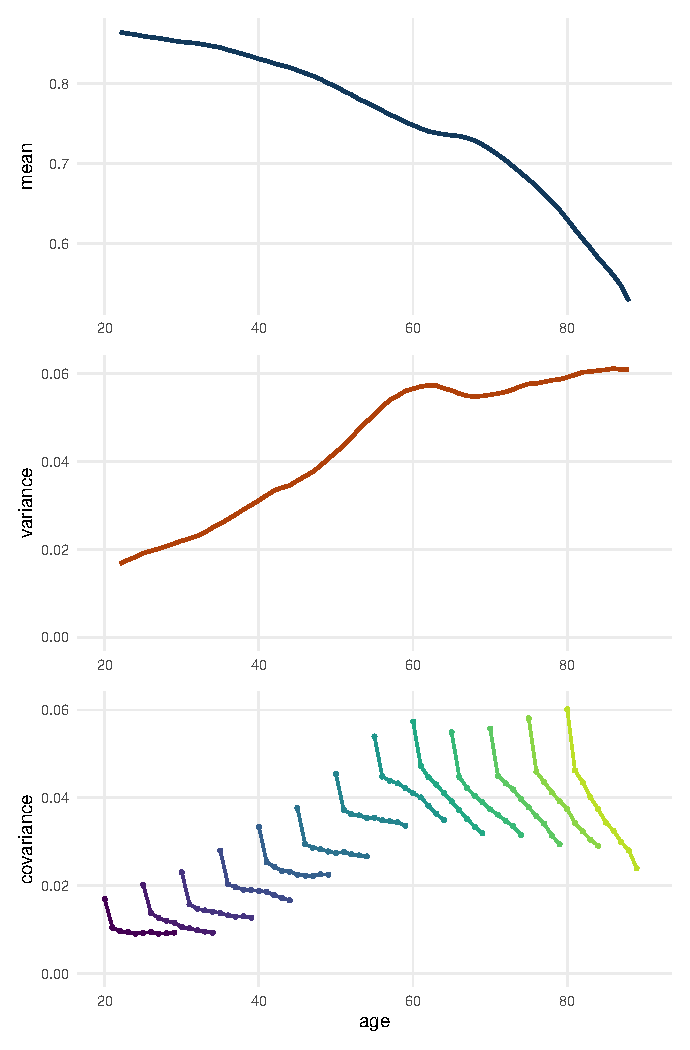
\includegraphics[width = 0.52 \linewidth]{emp_fig_v6_grid}
\end{figure}

\subsection{From observed moments to deterministic heterogeneity}

\begin{itemize}
\item Every observed level covariance splits into a between-type part and a noise part:
\begin{equation}
\Cov(h_s,h_t) \;=\; \Cov_j\bigl(\bar h_{j,s},\,\bar h_{j,t}\bigr) \;+\; \Cov(u_{i,s},u_{i,t}).
\label{eq:split}
\end{equation}
\item The returns need exactly the between-type part: $P(r)$ is built from the between-type variances $\Var_j(\bar h_{j,a})$ and covariances $\Cov_j(\bar h_{j,a},\bar h_{j,r-1})$, while observation delivers the sum.
Identification therefore means choosing cells where the noise term is zero or has a known shape.
\item In the linear case the between-type part is $V_H+(s+t)C_{Hd}+st\,V_d$ (Section~\ref{sec:linear}); the proposition only requires linearity over the waves used (A1).
\item Figure~\ref{fig:surfdata} is the object itself, in the data: every cell is one equation of the inversion.
\end{itemize}

\begin{figure}[H]
	\caption{The covariance surface of the primary measure, in five-year blocks. The diagonal is outlined; cells more than fourteen years off the diagonal are empty by construction - the panel is fifteen waves.}
	\label{fig:surfdata}
	\centering
	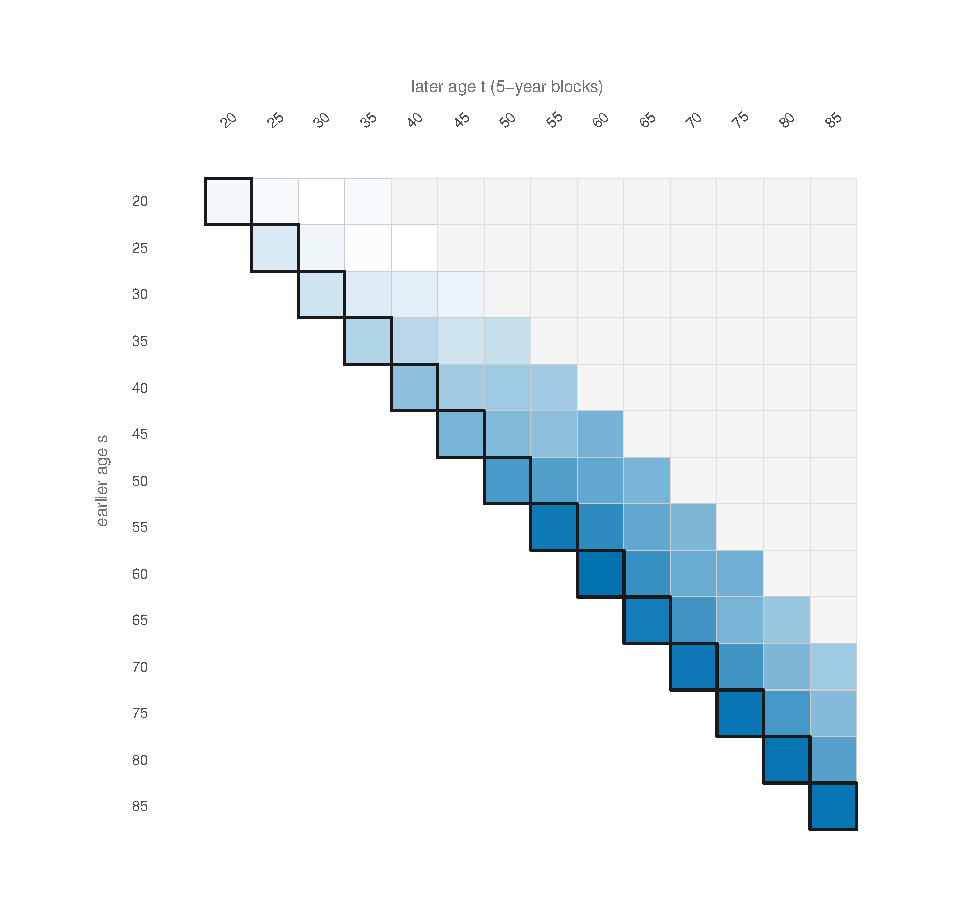
\includegraphics[width = 0.62 \linewidth]{emp_fig_v6_heatmap}
\end{figure}

The variances alone - the diagonal of the covariance matrix - are the objects that enter costs, but they are not enough, for two reasons.

\begin{enumerate}
\item If the noise variances are unrestricted, the diagonal identifies nothing at all: pure noise reproduces any variance profile exactly.
\item When the noise variance is stationary, the diagonal still cannot separate the type level $V_H$ from the noise: they enter every diagonal cell only as the bundle $V_H+\sigma^2_u$.
\end{enumerate}
\begin{itemize}
\item Figure~\ref{fig:twoworlds} illustrates this: the two worlds share every cross-section, and so every diagonal cell, and differ only off the diagonal.
\item Restoring identification needs a restriction on how the noise variance moves with age, and at least one off-diagonal cell. Lemma~\ref{lem:diag} in Appendix~\ref{app:props} states both precisely.
\end{itemize}

\noindent\textbf{Assumptions.}
\begin{itemize}
\item[A1.] (Window linearity) $d_{j,a}=d_j$ over the waves used.
\item[A2.] (Orthogonality) $\E[u_{i,a}\mid H_i,d_i]=0$ for all $a$. (allows type-specific shock variances.)
\item[A3.] (Noise distribution) Case dependent.
\end{itemize}

\subsection{The forces behind identification}\label{sec:forces}


Identification rests on a small number of forces, and each lives in a different region of the covariance matrix. The starting point is the rule of Section~\ref{sec:triad}: only what is carried from one wave to the next can produce covariance between waves.
The deterministic part is carried for ever.
Noise is carried according to its memory.
Momentary noise is not carried at all.\footnote{In derivative language, writing $C(s,t)=\Cov(h_s,h_t)$: the derivative along the diagonal (the slope of the variance profile) mixes the drift in the noise variance with the deterministic terms, and is clean only when the noise variance is stationary; the partial derivative in $t$ at fixed $s$ is a row read, equal to $C_{Hd}+rV_d$ wherever the noise is absent or has died; and the cross derivative $\partial^2C/\partial s\,\partial t$ - discretely the double difference, algebraically $\Cov(\Delta h_s,\Delta h_t)$ - isolates the curvature $V_d$, because the tilt cancels.}

\subsubsection*{The diagonal}

\begin{itemize}
\item Every component adds variance, so every component appears in $V(a)$. On its own the diagonal separates nothing, unless the stochastic component has stationary variance.
\item The force that makes it useful is stationarity: if the noise contributes the same variance at every age, differences of $V(a)$ remove it completely.
\item What survives differencing is the deterministic part, because it grows with age in a known way: $C_{Hd}$ adds a linear term and $V_d$ a quadratic one, so the slope and curvature of the diagonal are $C_{Hd}$ and $V_d$.
\item This force ignores memory: any noise with constant variance drops out of the differences, so persistence never touches what the diagonal delivers.
\item The force fails when $v_a$ moves with age: on the diagonal alone, a drifting noise variance cannot be told apart from deterministic growth.
\end{itemize}

\subsubsection*{The first row}

\begin{itemize}
\item The force here is separation by shape. Fix wave 0 and move the later wave: the deterministic part contributes a straight line, $V_H+aC_{Hd}$, because $H$ and $d$ are carried unchanged.
\item Carried noise contributes a shape of its own, and the shape is what identifies the process.
Under AR(1) it is a geometric decay $\rho^a v_0$, a share $\rho$ surviving each step; under an MA($q$) it dies after $q$ steps; under a random walk it is flat.
\item A line and a geometric decay cannot imitate each other, which is what splits the level from the noise and measures the memory. The exception is the flat case, and that is the limit below.
\item A component carried to no other cell at all - a pure one-period spike - is invisible to the row entirely; the gap between the diagonal and the row's back-extrapolation is what measures it.
\item The anchor $V(0)$ is part of the row: it is the $a=0$ point of the same function. That is why the row's second differences can remove the line.
\item The force has a limit: as $\rho\to1$ the decay flattens into a constant and merges with $V_H$.
This is the bundle - a permanent shock, once landed, is carried exactly like a type level (``what stays'', Section~\ref{sec:triad}).
\item The row never contains $V_d$: the curvature term is $st\,V_d$, and on the first row $s=0$. Whatever the row cannot deliver has to come from the interior.
\end{itemize}

Figure~\ref{fig:rowsdata} shows this force in the data: the rows of the primary measure's matrix, leaving the diagonal at five-year base ages.
The row from base age 35 drops off the diagonal - the spike dying - and then runs essentially flat: a line with almost no slope.
The row from base age 70 drops and then keeps falling.
One stationary noise process cannot produce both, because the same fade would have to appear at every base age.
Either the noise moves with age, or the line's own slope has changed sign - which is the local reading of Section~\ref{sec:back}.

\begin{figure}[H]
	\caption{Rows of the covariance matrix (primary measure), each starting on the diagonal at its own base age and running nine years. The initial drop is the one-year spike; what remains is the line plus any carried noise.}
	\label{fig:rowsdata}
	\centering
	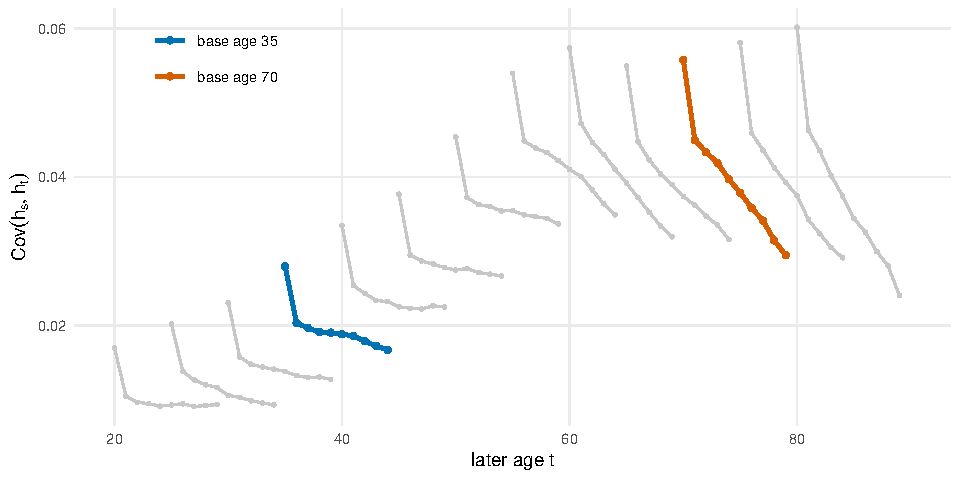
\includegraphics[width = 0.72 \linewidth]{emp_fig_v6_rowsfull}
\end{figure}

\subsubsection*{The interior}

\begin{itemize}
\item $V_d$ multiplies $st$, so it appears on the diagonal (as $a^2V_d$) and in the interior (as $st\,V_d$), but never in the first row.
\item When the diagonal is readable, its curvature gives $V_d$ and the interior is spare. When it is not, the interior is the only place left.
\item With the row solved, two interior cells contain exactly two unknowns, $V_d$ and $v_1$: the noise they carry, $\rho^{\,t-s}v_s$, uses the memory the row has already measured.
\item Every further cell is spare capacity: an overidentifying test, or the budget for relaxing an assumption - which is what the cases below spend it on.
\end{itemize}

\begin{table}[H]
\caption{The three regions and their forces}
\label{tab:forces}
\centering
\footnotesize
\begin{tabular}{@{}lL{4.1cm}L{3.2cm}L{3.4cm}@{}}
\toprule
\textbf{Region} & \textbf{Force} & \textbf{Delivers} & \textbf{Fails when} \\
\midrule
Diagonal $V(a)$ & stationary noise cancels in differences & $C_{Hd}$, $V_d$ & $v_a$ moves with age \\
First row $C_0(a)$ & a line cannot mimic a geometric decay & level split; $\rho$ & $\rho\to1$: noise becomes permanent and merges with the level \\
Interior & $st\,V_d$ needs both indices to move & $V_d$ when the diagonal cannot be read; tests otherwise & - \\
\bottomrule
\end{tabular}
\end{table}

\begin{itemize}
\item The policy mapping follows the regions: the diagonal prices the uniform returns (Section~\ref{sec:back}), the row provides the split that targeting needs (Result~\ref{res:target}), and the interior completes the general case and supplies the tests.
\end{itemize}

\subsection{Four cases: the two curves and the interior}\label{sec:cases}

Two functions of the data organise everything below:
\begin{equation}
V(a)\equiv\Var(h_a),
\qquad
C_0(a)\equiv\Cov(h_0,h_a),
\qquad\text{with } C_0(0)=V(0).
\label{eq:curves}
\end{equation}
$V(a)$ is the diagonal of the covariance matrix and $C_0(a)$ is its first row.
The interior cells $\Cov(h_s,h_t)$ with $s\ge1$ are the third region: they are where $V_d$ has to come from once the diagonal can no longer be read, and elsewhere they are overidentifying checks.
Section~\ref{sec:forces} explains what each region can do; the formulas that recover a case's parameters we call the \emph{reads} of that case.
Proofs are in Appendix~\ref{app:props}.

\begin{proposition}[Identification within the AR-plus-spike class]\label{prop:main}
Assume A1-A2 and let the noise satisfy
$\Cov(u_s,u_t)=\rho^{\,t-s}v_s+\mathbf{1}\{s=t\}\,\sigma^2_{\varepsilon,s}$ for $s\le t$, with $\rho\in[0,1)$: a carried component with memory $\rho$ and variances $v_s$, plus a one-period spike $\sigma^2_{\varepsilon,s}$.
Then:
\begin{itemize}
\item[(i)] five waves identify $V_H$, $C_{Hd}$, $V_d$, $\rho$ and both noise variances at the waves used (the last wave's two components only in sum);
\item[(ii)] with the spike absent, four waves suffice (Case 3); with both noise variances stationary, four waves suffice (Case 4);
\item[(iii)] with the spike absent and the carried variance stationary, three waves suffice, whatever the memory $\rho$ (Cases 1-2);
\item[(iv)] if in addition $C_{Hd}=0$ and the noise is memoryless, two waves suffice.
\end{itemize}
The explicit reads are given by the four cases below.
\end{proposition}

\begin{itemize}
\item Some restriction on the noise is necessary (here: a carried component plus a one-period spike). Identification needs at most as many parameters as there are moments, and an unrestricted noise covariance already uses all of them: with $T$ waves there are $T(T+1)/2$ covariance moments and exactly that many free noise parameters.
\item Structure on how the noise is carried - here one memory parameter and one variance per wave - is what leaves room for the deterministic block.
Lemma~\ref{lem:diag} makes the same point on the diagonal.
\item Part (iii) is the substantive one: with a stationary carried variance and no spike, memory costs nothing in waves. What raises the requirement to four is not persistence but either a carried variance that moves with age (Case 3) or a component the row cannot see at all (Case 4).
\end{itemize}

\paragraph{Case 1: i.i.d.\ noise, stationary variance $\sigma^2_u$ (three waves).}
The two curves are
\begin{equation}
V(a)=V_H+2aC_{Hd}+a^2V_d+\sigma^2_u,
\qquad
C_0(a)=V_H+aC_{Hd}\quad(a\ge1).
\end{equation}
The curvature and slope of the diagonal give the evolution parameters,
\begin{equation}
V_d=\tfrac12\bigl[V(2)-2V(1)+V(0)\bigr],
\qquad
C_{Hd}=\tfrac12\bigl[V(1)-V(0)-V_d\bigr],
\label{eq:profilereads}
\end{equation}
and one row cell splits the level from the noise: $V_H=C_0(1)-C_{Hd}$, $\sigma^2_u=V(0)-V_H$.

\begin{figure}[H]
	\caption{Illustration of Case 1: the two curves}
	\label{fig:case1curves}
	\centering
	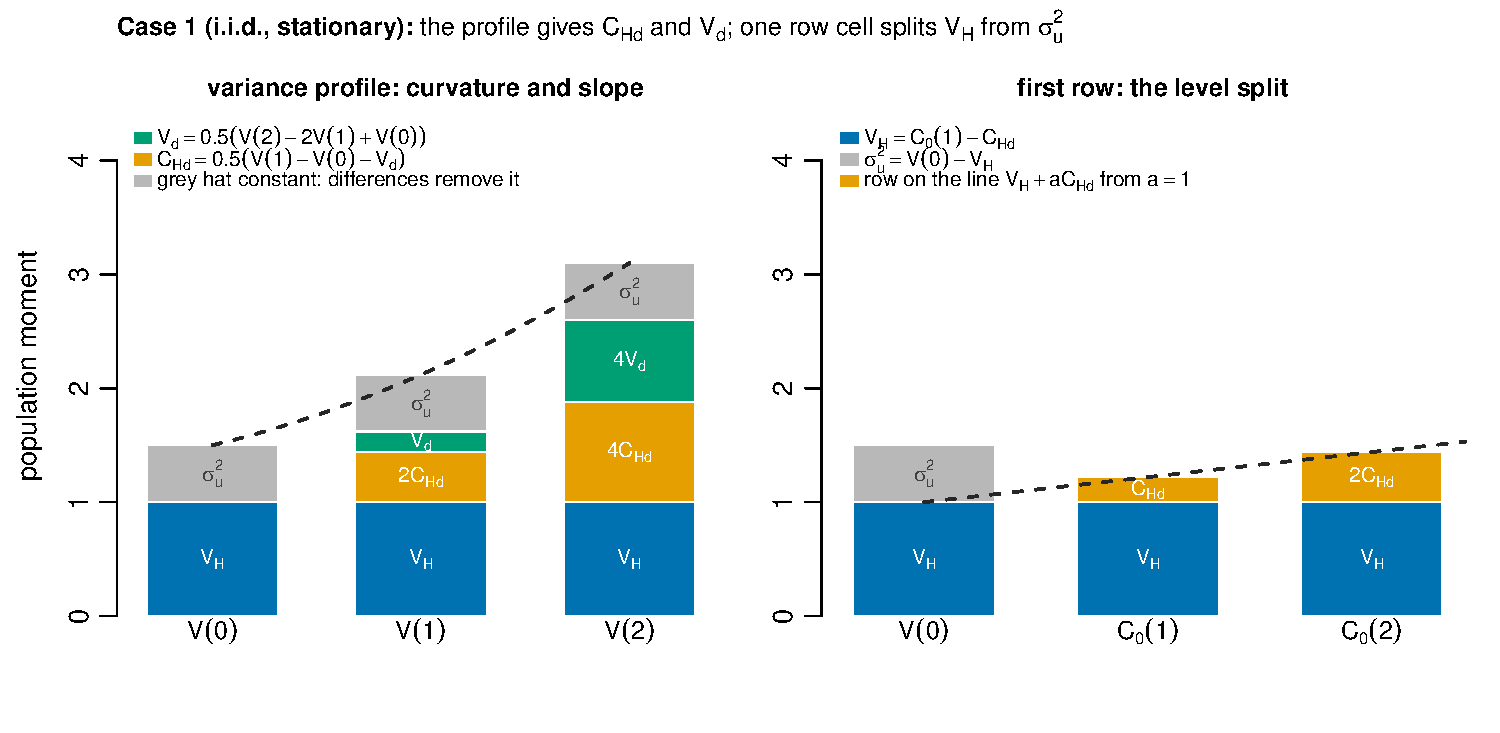
\includegraphics[width = 0.82 \linewidth]{figures/fig_case1_curves}
\end{figure}

\begin{itemize}
\item The noise adds the same amount to every variance, so it cancels in the differences that give $C_{Hd}$ and $V_d$ (Figure~\ref{fig:case1curves}).
\item Benchmark: imposing $C_{Hd}=0$ reduces this to two waves, with $V_d=V(1)-V(0)$ - part (iii) of the proposition.
\end{itemize}

\paragraph{Case 2: AR(1) noise, stationary variance (three waves).}
Let $u_{i,a}=\rho\,u_{i,a-1}+\eta_{i,a}$ with $\rho\in[0,1)$ and $u_{i,0}$ drawn from the stationary distribution. Then $V(a)$ is as in Case 1 and
\begin{equation}
C_0(a)=V_H+aC_{Hd}+\rho^a\sigma^2_u .
\end{equation}
The diagonal identification \eqref{eq:profilereads} is unchanged, so the tilt is already known; remove it from the row.
The \emph{detilted row} $\tilde C_0(a)\equiv C_0(a)-aC_{Hd}$ equals $V_H+\rho^a\sigma^2_u$, and its successive drops shrink by a factor $\rho$ at each step:
\begin{equation}
\rho=\frac{\tilde C_0(1)-\tilde C_0(2)}{\tilde C_0(0)-\tilde C_0(1)},
\qquad
\sigma^2_u=\frac{\tilde C_0(0)-\tilde C_0(1)}{1-\rho},
\qquad
V_H=\tilde C_0(0)-\sigma^2_u .
\label{eq:fade}
\end{equation}

\begin{figure}[H]
	\caption{Illustration of Case 2: the two curves}
	\label{fig:case2curves}
	\centering
	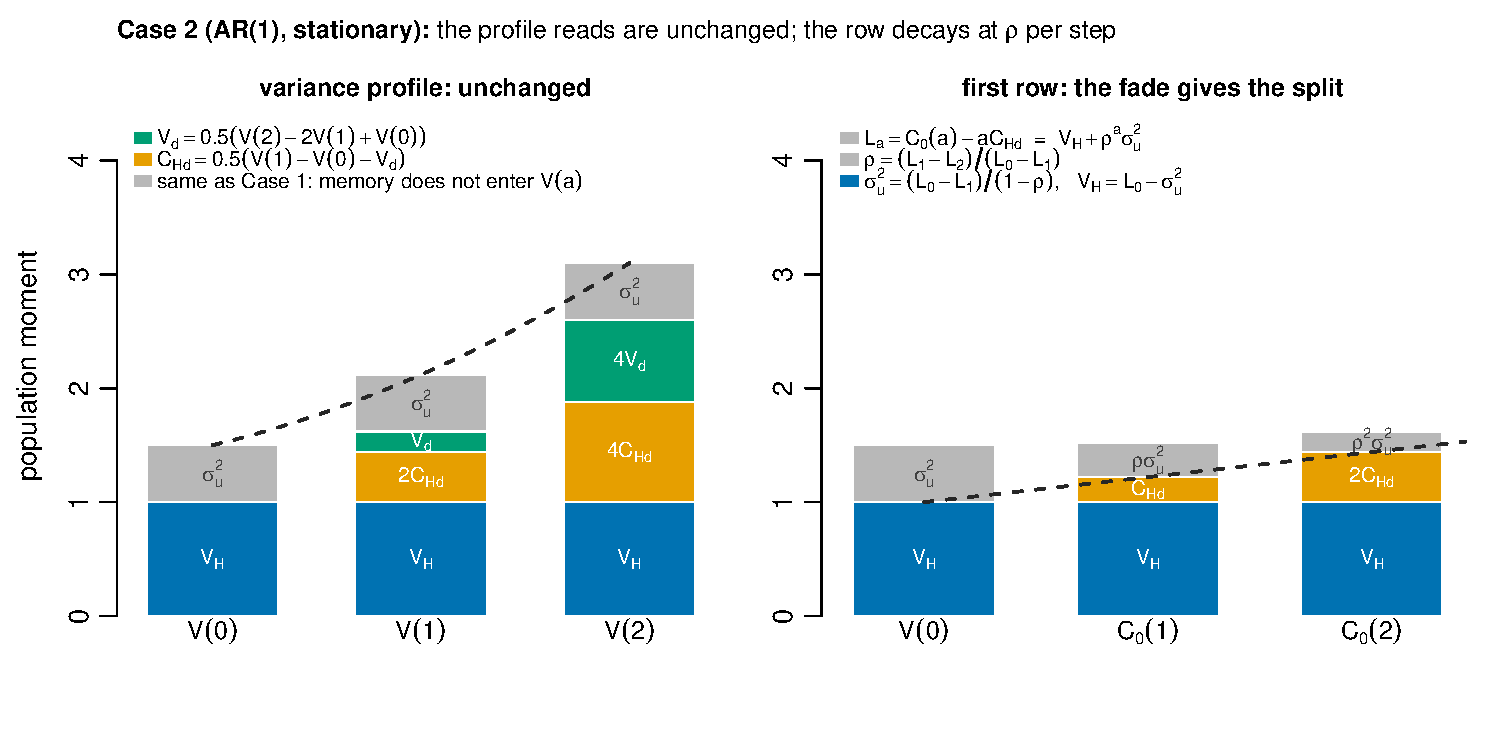
\includegraphics[width = 0.82 \linewidth]{figures/fig_case2_curves}
\end{figure}

\begin{itemize}
\item The diagonal identifications are identical to Case 1: noise memory never enters $V(a)$ while its variance is stationary.
\item The row cells sit above the line $V_H+aC_{Hd}$ by $\rho^a\sigma^2_u$; two shrinkage steps give $\rho$ (Figure~\ref{fig:case2curves}).
\end{itemize}

The same read on the data: three ages three years apart, pooled over base ages within a window, with $\rho$ profiled and the rest solved by least squares.
Figure~\ref{fig:case2data} draws the fitted decomposition of all six moments in every window where the answer is a valid covariance matrix.

\begin{figure}[H]
	\caption{Case 2 on the data (primary measure): three ages three years apart, the six moments and their fitted decomposition, in the windows where the deterministic block is a valid covariance matrix. The young window (25-41) fails and is not drawn.}
	\label{fig:case2data}
	\centering
	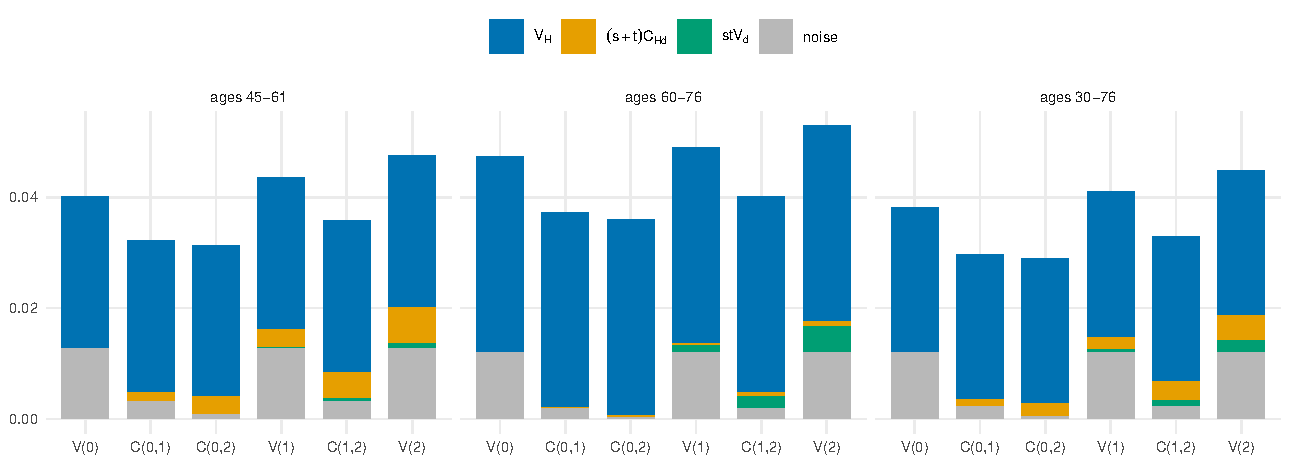
\includegraphics[width = 0.98 \linewidth]{emp_fig_v6_case2}
\end{figure}

\begin{itemize}
\item In the mid-life window (45-61) the read delivers the full parameter set: $\rho=0.63$, a level/noise split of $V_H=0.027$ against $\sigma^2_u=0.013$, and visible evolution terms with $\Corr(H,d)=0.64$.
\item The window matters: at 60-76 the evolution terms nearly vanish (the diagonal is flat there), and in the young window (25-41) the read fails - $V_d$ comes back negative, which is why it is not drawn.
\item All fits match their six cells to within a third of a percent; the sign and size of the small $C_{Hd}$ are the fragile part, taken up below and in Appendix~\ref{app:localpass}.
\end{itemize}

\paragraph{Case 3: AR(1) noise, age-specific variances $v_a$ (four waves).}
The noise layer is
\begin{equation}
\Cov(u_s,u_t)=\rho^{\,t-s}\,v_s
\qquad (s\le t),
\label{eq:case3noise}
\end{equation}
so
\begin{equation}
V(a)=V_H+2aC_{Hd}+a^2V_d+v_a,
\qquad
C_0(a)=V_H+aC_{Hd}+\rho^a v_0 .
\end{equation}
The diagonal now identifies nothing (Lemma~\ref{lem:diag}(i)), so the row must find both the line and the decay: four cells, four parameters.
Second differences of the row remove the line and leave only the decay, so their ratio is the memory,
\begin{equation}
\rho=\frac{C_0(3)-2C_0(2)+C_0(1)}{C_0(2)-2C_0(1)+C_0(0)},
\qquad
v_0=\frac{C_0(2)-2C_0(1)+C_0(0)}{(1-\rho)^2},
\label{eq:rowreads3}
\end{equation}
and then $V_H=V(0)-v_0$ and $C_{Hd}=C_0(1)-C_0(0)+(1-\rho)v_0$.
Two interior cells give $V_d$: with $(V_H,C_{Hd},\rho)$ known, $\Cov(h_1,h_2)$ and $\Cov(h_1,h_3)$ leave exactly the two unknowns $(V_d,v_1)$ (closed form in Appendix~\ref{app:props}, Case 3).
The remaining variances follow from the diagonal, $v_a=V(a)-V_H-2aC_{Hd}-a^2V_d$.

\begin{figure}[H]
	\caption{Illustration of Case 3: the two curves, then the interior}
	\label{fig:case3curves}
	\centering
	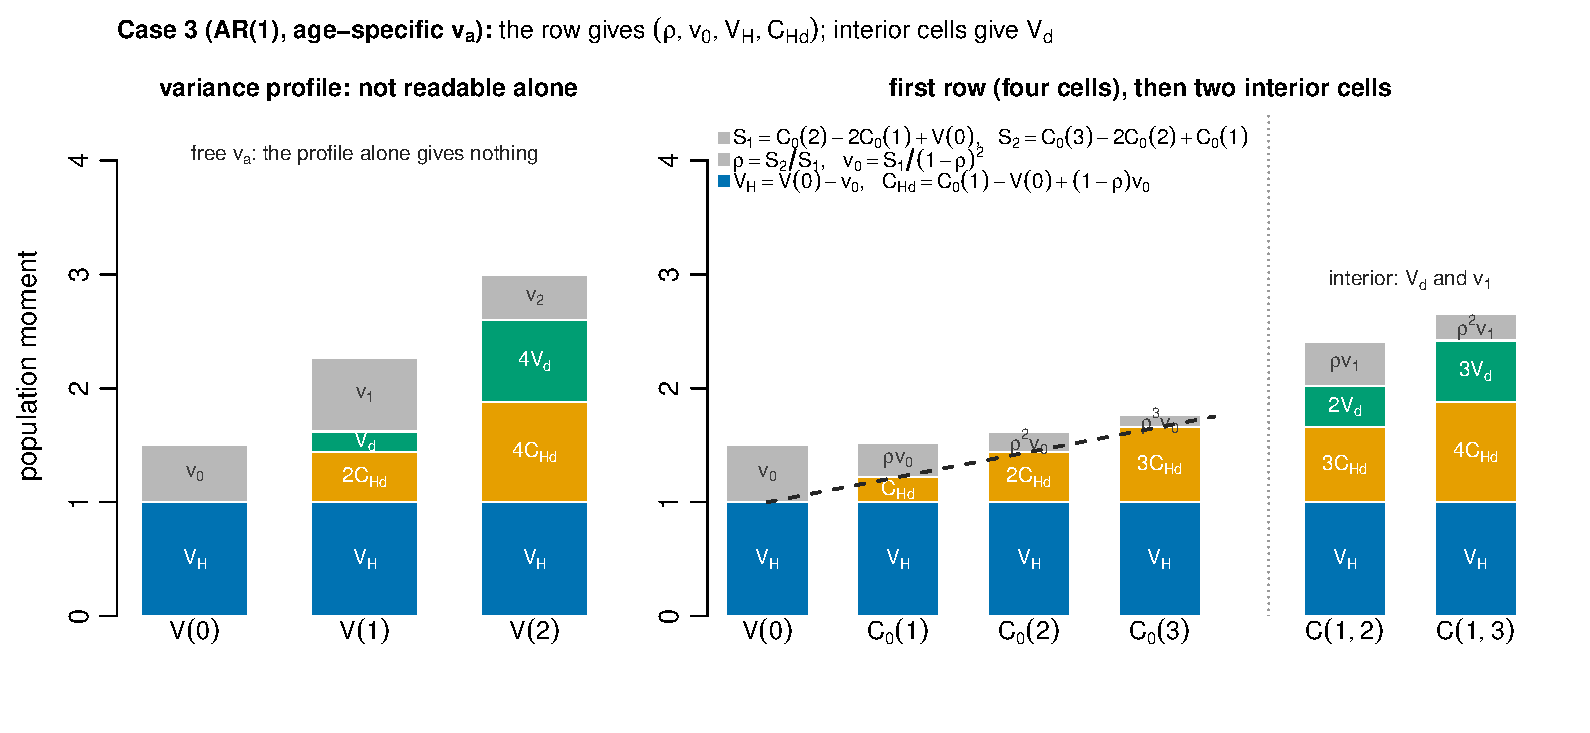
\includegraphics[width = 0.88 \linewidth]{figures/fig_case3_curves}
\end{figure}

\begin{itemize}
\item In Case 2 the diagonal supplied the line and the row had only to find the fade. Here the diagonal supplies nothing, so the row must find the line and the fade at once, hence the second differences rather than first (Figure~\ref{fig:case3curves}).
\item Case 3 nests Cases 1 and 2: $\rho=0$ with free $v_a$ is the denoising case (Appendix~\ref{app:surface}); constant $v_a$ is Case 2; $\rho=1$ is the random walk.
\item If $v_a$ is linear in $a$, the noise is a random walk with constant innovation variances; the $\rho\to1$ limit is discussed in Section~\ref{sec:forces} and treated in full in Proposition~\ref{prop:F1}.
\end{itemize}

\paragraph{Case 4: AR(1) noise plus one-period measurement error (four waves).}
Split the shock into a carried part and a momentary part, $u_{i,a}=w_{i,a}+\varepsilon_{i,a}$: $w$ is AR(1) with memory $\rho$ and stationary variance $\sigma^2_w$, and $\varepsilon$ is measurement error - i.i.d.\ with variance $\sigma^2_\varepsilon$, shared with no other cell.
Then
\begin{equation}
V(a)=V_H+2aC_{Hd}+a^2V_d+\sigma^2_w+\sigma^2_\varepsilon,
\qquad
C_0(a)=V_H+aC_{Hd}+\rho^a\sigma^2_w\quad(a\ge1).
\end{equation}
The total noise variance is constant, so the diagonal reads \eqref{eq:profilereads} survive unchanged.
The spike appears in every diagonal cell and in no off-diagonal cell, so the row is blind to it - and Case 2's fade read breaks, because its first drop $\tilde C_0(0)-\tilde C_0(1)$ is inflated by $\sigma^2_\varepsilon$.
The repair uses only drops the spike cannot touch:
\begin{equation}
\rho=\frac{\tilde C_0(2)-\tilde C_0(3)}{\tilde C_0(1)-\tilde C_0(2)},
\qquad
\sigma^2_w=\frac{\tilde C_0(1)-\tilde C_0(2)}{\rho(1-\rho)},
\qquad
V_H=\tilde C_0(1)-\rho\,\sigma^2_w,
\label{eq:case4reads}
\end{equation}
and the spike is the anchor's excess over the fade, $\sigma^2_\varepsilon=V(0)-V_H-\sigma^2_w$.
Needing $\tilde C_0(3)$ is what makes this a four-wave case.

\begin{figure}[H]
	\caption{Illustration of Case 4: the fade is read from off-diagonal drops only; the spike lives on the diagonal alone}
	\label{fig:case4curves}
	\centering
	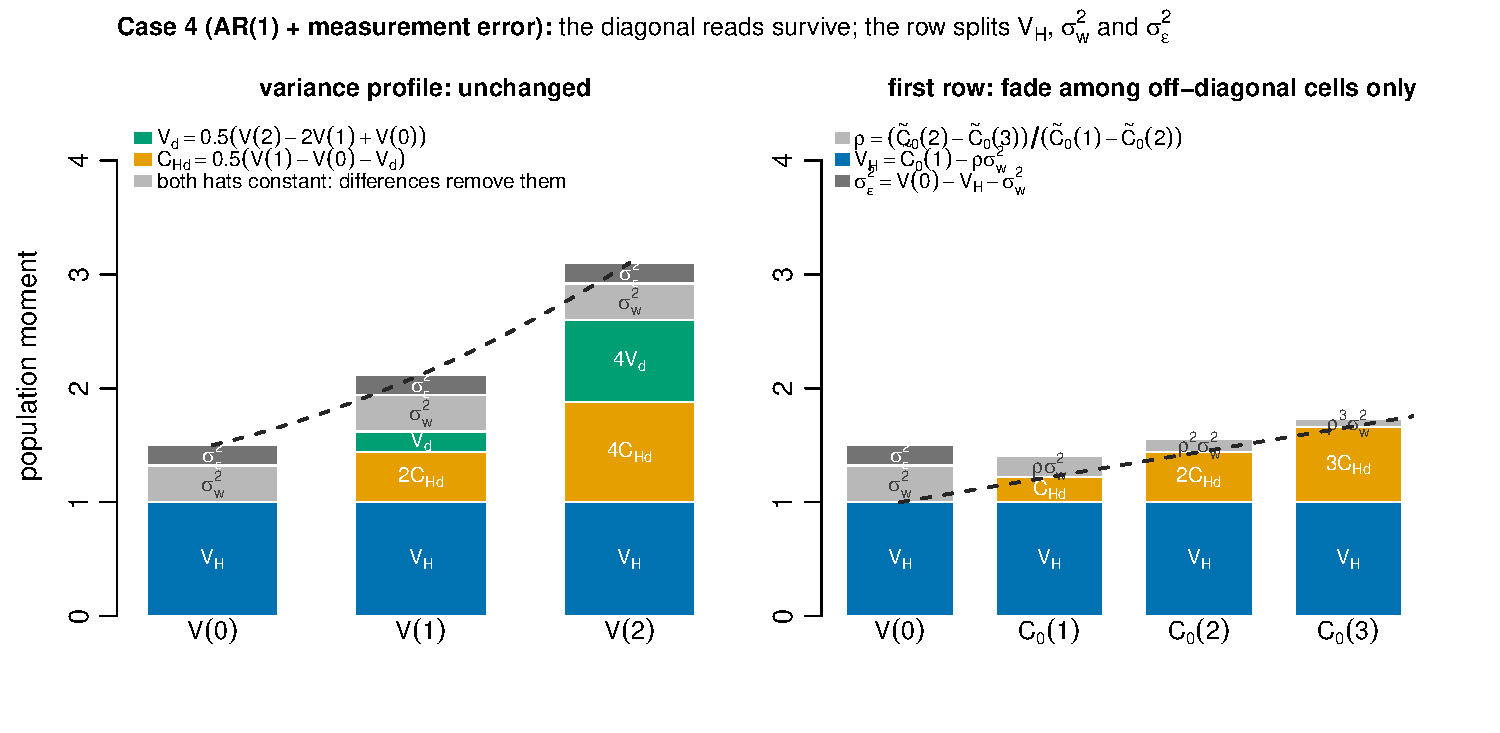
\includegraphics[width = 0.88 \linewidth]{figures/fig_case4_curves}
\end{figure}

\begin{itemize}
\item The split needs memory: at $\rho=0$ both components die in one period and only their sum is identified.
Measurement error is separable from genuine transitory health only because the genuine part is carried.
\item Three waves are not enough despite the parameter count (six moments, six parameters): the interior cell is implied by the diagonal differences, so the map is rank-deficient - the fourth wave is genuinely needed.
\item This is the case that makes the treatment-side caveat of Section~\ref{sec:compare} operational: $\sigma^2_\varepsilon$ is exactly the object excluded from $\Var(h_a)$ in $T(r)$, while $\sigma^2_w$ stays in.
\item Sibling to Case 3: each spends the fourth wave on one relaxation - a drifting carried variance there, the spike here.
Both at once is the five-wave general member of the proposition.
\item Nesting: $\sigma^2_\varepsilon=0$ is Case 2; $\rho\to1$ is the random walk plus measurement noise of Proposition~\ref{prop:F1}.
\item On the data the case is admissible where Case 2 is (from age 60): there the spike is a sixth to a fifth of the variance and the carried part is slow, $\rho\approx0.9$ (full record in the companion \texttt{testing\_metrics.tex}).
The estimation-side counterpart is the bundle fit of Appendix~\ref{app:localpass}: with $\rho$ near one, the carried part is folded into the level rather than estimated.
\end{itemize}

\paragraph{Estimation and checks.}
\begin{itemize}
\item The ratios \eqref{eq:fade} and \eqref{eq:rowreads3} divide small differences: exact in population, noisy in samples.
\item In estimation the parameters would be chosen to fit all cells jointly (minimum distance, as in the earnings-dynamics literature); the closed forms above are the just-identified special cases that use exactly as many cells as parameters.
\item Minimum distance works because the map is invertible, which is what the proposition establishes, and the cases say which cells carry which parameter - hence what drives precision.
\item Every cell a case does not use is an overidentifying check.
\end{itemize}

\textbf{Linear-regression representation.} Every case can equivalently be expressed through individual growth regressions: OLS of $h_{i,a}$ on $(1,a)$ person by person, keeping intercepts, slopes and residuals.
The coefficient moments are an invertible linear transform of the level moments, and the transform depends only on which waves are used, not on the noise, so the two representations always carry the same information.
What is case-specific is the correction for noise, not the representation (Appendix~\ref{app:growth}).

\subsection{Back to the returns}\label{sec:back}

In the linear case of Section~\ref{sec:linear}: $h_{i,a}=H_i+a\,d_i+u_{i,a}$, the type mean paths are straight lines, $\bar h_{j,a}=H_j+a\,d_j$, and Proposition~\ref{prop:main} has just recovered the parameters $(V_H,V_d,C_{Hd}$ and the noise parameters$)$ of \eqref{eq:forwardmap} from the covariance matrix. Substituting back into the returns of Section~\ref{sec:cost}:

\begin{itemize}
\item The preventable decline becomes window length times the type's own slope, $\bar h_{j,r-1}-\bar h_{j,a}=-(a-r+1)\,d_j$, so the between-type channel of \eqref{eq:Ppop} reduces to identified objects,
\begin{equation}
\Cov_j\bigl(1-\bar h_{j,a},\,\bar h_{j,r-1}-\bar h_{j,a}\bigr)=(a-r+1)\bigl(C_{Hd}+aV_d\bigr),
\end{equation}
and the mean path is $\bar h_a=\bar H+a\bar d$, so
\begin{equation}
P(r)=2\sum_{a=r}^{\bar a}\Bigl[\bigl(1-\bar h_a\bigr)\bigl(\bar h_{r-1}-\bar h_a\bigr)+(a-r+1)\bigl(C_{Hd}+aV_d\bigr)\Bigr].
\label{eq:Plin}
\end{equation}
Compounding ($C_{Hd}>0$) raises the return, but even with $C_{Hd}=0$ the term $aV_d$ is positive.
Summing the second term over $a$ gives the single combination $K(r)=A(r)C_{Hd}+B(r)V_d$ that a fixed starting age needs.\footnote{$K(r)$ is not cheaper to identify than the pair: no two-wave combination is proportional to it, so it costs the same moments as $(C_{Hd},V_d)$, and the timing profile needs the two separately.
Appendix~\ref{app:prev} states this and gives the weights $A(r)$, $B(r)$.}
\item The three channels of \eqref{eq:covdecomp} are now visible in the parameters: the pathway margin is $(a-r+1)C_{Hd}$, the persistence margin $(r-1)(a-r+1)V_d$, and the accumulation margin $(a-r+1)^2V_d$.
\item The two $V_d$ pieces sum to $(a-r+1)a\,V_d$, so the life-course decomposition and \eqref{eq:Plin} are the same object; a later start puts more of the $V_d$ term into persistence and less into accumulation.
\item The mix shifts with $r$ as each sum is exposure time times the gap-decline covariance, $(a-r+1)(C_{Hd}+aV_d)$, where the level $H$ in the gap contributes $C_{Hd}$ and the accumulated slope $a\,d$ contributes $aV_d$. Starting later drops the low-$a$ terms, where slope heterogeneity has had little time to open gaps, and so tilts the mix toward $V_d$.
\item Treatment side: the parameters enter only through the total variance, so no decomposition is needed:
\begin{equation}
	T(r)=2\sum_{a\ge r}\Bigl[(1-\bar h_a)^2+\underbrace{V_H+2aC_{Hd}+a^2V_d+v_a}_{=\,\Var(h_a)\text{, directly observable}}\Bigr].
\label{eq:Tlin}
\end{equation}
\item Every case supplies all the inputs to \eqref{eq:Plin} and \eqref{eq:Tlin}: Cases 1 and 2 from three waves, Case 3 from four.
In Cases 1-2 the inputs come from the diagonal, so repeated cross-sections suffice; Case 3 needs the first row and two interior cells, and so a panel.
\end{itemize}

\paragraph{The local reading.}
\begin{itemize}
\item Nothing above requires one line for life: A1 is linearity over the waves used, so the parameters are local to the window around the base age.
Define the local level-change covariance $C_{Hd}(a)\equiv\Cov_j(\bar h_{j,a},\,d_j)$; within the window, $C_{Hd}(a)=C_{Hd}+a\,V_d$.
\item The curves of Section~\ref{sec:ident} read the local object directly.
The one-step growth of the deterministic variance is $\Var_j(\bar h_{j,a+1})-\Var_j(\bar h_{j,a})=C_{Hd}(a)+C_{Hd}(a+1)$: the variance rises exactly while the local covariance is positive, and falls once it turns negative.
\item A variance profile that turns over therefore requires $C_{Hd}(a)$ to change sign.
The global linear model cannot produce it - there $C_{Hd}(a)=C_{Hd}+aV_d$ only increases.
Figure~\ref{fig:threepanel} shows the cross-sectional version of this fact; how much of it is the local covariance itself and how much is composition - who survives to be measured at each age - is the empirical section's question, with a first pass parked in Appendix~\ref{app:localpass}.
\item Beyond the reach of the noise, the row anchored at $s$ falls or rises at rate $C_{Hd}(s)$; where the row runs past the window, its slope at lag $k$ is the covariance of the base-age level with the change at the age traversed, $\Cov_j(\bar h_{j,s},\,d_{j,s+k})$ - the rows are forward-looking.
\item The between-type channel of \eqref{eq:Plin} is the exposure-weighted sum of the local objects: each summand is $(a-r+1)\,C_{Hd}(a)$.
The return never needed the global parameters as such; the linear window is one way of extrapolating the local sequence.
\item Figure~\ref{fig:localchart} is the local reading on the data: the denoising solve of the triple at three base-age windows.
$V_H$ grows as shocks accumulate into the level; the covariance term starts near zero and turns negative - the compression the rows of Figure~\ref{fig:rowsdata} show directly.
\item The sign of the small covariance term is where the noise treatment bites: the Case 2 read of Figure~\ref{fig:case2data} holds the noise variance fixed and finds it positive in mid-life, while the denoising solve lets the noise move and finds it negative from mid-life on.
Which is right depends on the noise process, and settling that is the empirical section's job.
\item A first empirical pass at $C_{Hd}(a)$, and the estimation issues it raises, is parked in Appendix~\ref{app:localpass}.
\end{itemize}

\begin{figure}[H]
	\caption{The local triple in the data (primary measure): the denoising solve on twelve-year windows at three life stages. Each panel has its own scale.}
	\label{fig:localchart}
	\centering
	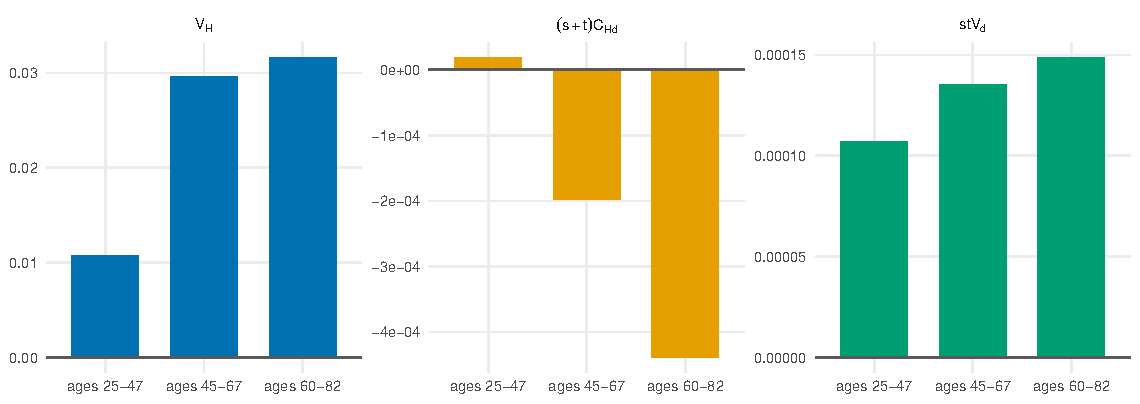
\includegraphics[width = 0.88 \linewidth]{emp_fig_v6_local}
\end{figure}

\begin{itemize}
\item The returns sum to the end of the horizon, while the window identifies the local parameters.
Carrying them forward is an extrapolation, and the linear window is its maximal-persistence case: the slope a person carries today is the slope they keep.
\item If slopes mean-revert across windows, the compounding terms shrink, and the long-horizon return falls with the persistence of the slope.
That persistence is an estimand, not a convention: it lives in the long-lag cells of the covariance matrix.
\end{itemize}

\jnote{With enough waves the cross-window persistence of $d$ is estimable from long-lag interior cells; the returns section should eventually report long-horizon returns under the estimated persistence rather than the perfect-persistence default.}

Table~\ref{tab:dict} collects the dictionary from policy objects to the moments and data that deliver them.

\begin{table}[H]
\caption{What each policy object needs}
\label{tab:dict}
\centering
\small
\begin{tabular}{@{}L{4.3cm}L{4.6cm}L{4.6cm}@{}}
\toprule
\textbf{Policy object} & \textbf{Moments needed} & \textbf{Data} \\
\midrule
Healthcare cost; treatment return $T(r)$ & mean path; $\Var(h_a)$ & cross-sections \\
Prevention return $P(r)$, fixed $r$ & mean path; one combination of $C_{Hd}$ and $V_d$ & 3 cross-sections if the noise variance is stationary; a 4-wave panel if it drifts \\
Timing profile $r\mapsto P(r)$ & mean path; $C_{Hd}$ and $V_d$ separately & as above \\
Targeting on $h_0$ (Result~\ref{res:target}) & first row; the level/noise split & panel \\
Targeting gain, type vs.\ uniform (App.~\ref{sec:targeting}) & spread of $P_j$ across types & panel $+$ clusters \\
Targeting gain, type vs.\ level (App.~\ref{sec:targeting}) & how well the pre-policy level predicts $P_j$; noise in that level & panel $+$ clusters \\
%Timing of divergence & rolling-window $V_d(a)$, $C_{Hd}(a)$ & panel \\
\bottomrule
\end{tabular}
\end{table}

The two prevention rows need the same moments: identifying the combination is not cheaper than identifying the pair (Appendix~\ref{app:prev}).

Obviously, a panel is still useful where cross-sections suffice - it tests the stationarity the cross-sectional reads rely on, and delivers the level/noise split that targeting needs.

\jnote{Given that the $K(r)$ combination needs as many moments to identify as $C_{Hd}$ and $V_d$ do, we could merge the two $P(r)$ rows of this table into one.}

\paragraph{The framework in the data.}
Return to Figure~\ref{fig:threepanel}, with the section's machinery in hand.

\begin{itemize}
\item The variance rises steeply to about age 60 and then stops growing (the thin-celled tail past 80 is noisy), even as mean decline accelerates.
Under a stationary noise variance this says the local covariance $C_{Hd}(a)$ has reached zero by 60, and the one-year spike moves too little to change that reading (Appendix~\ref{app:localpass}).
\item The rows steepen with the base age, as in Figure~\ref{fig:rowsdata}: the old rows' sustained fall says the local covariance keeps falling past zero.
\item One caution before reading these curves as pure dynamics: part of the variance flattening is composition - the tails are thinned by who survives to be measured - and the split between genuine compression and composition, with selection, floors and cohort effects handled properly, is the empirical companion's job.
The framework's job here is only to show that its objects are visible, and readable, in the data.
\end{itemize}
%
%\textbf{Empirical counterparts.} Every object above is a sample moment. The checklist for the data section:
%\begin{itemize}
%\item the two curves $V(a)$ and $C_0(a)$, plotted from the data;
%\item the triangular heatmap of the whole covariance matrix;
%\item rows of the matrix at $s\ge1$, whose shape separates the noise processes (Figure~\ref{fig:rowreads});
%\item the ladder $D_k\equiv\Cov(\Delta h_t,\Delta h_{t+k})$: dip-then-flat, geometric rise or flat, which diagnoses the noise process from changes rather than levels (Appendix~\ref{app:props}, the $D_k$ ladder).
%\end{itemize}
%

\begin{comment}
%% =============================================================================
\section{Empirical roadmap and open points}
%% =============================================================================

\subsection{Roadmap}

\begin{itemize}
\item[1.] \textbf{Lag profile and covariance surface} (UKHLS): estimate $V_d$, $C_{Hd}$,
$\sigma^2$'s by minimum distance; run the overidentification and plateau-flatness tests.
Report the growth-regression representation alongside for
interpretability (Appendix~\ref{app:growth}).
\item[2.] \textbf{Rolling age windows}: age profiles $V_d(a)$, $C_{Hd}(a)$ - when does
deterministic divergence open? This is the timing-of-prevention question, answered with the
same machinery (and relaxing window linearity).
\item[3.] \textbf{Clustering} (partial $k$-means; Bayesian) as nonparametric estimation of
the $(H,d)$ support: compare between-cluster variance with moment-based $V_d$ - clustering
on realized paths selects on noise, so an overshoot is an overfitting diagnostic
(split-sample clustering as the fix); autocorrelation of within-cluster deviations as the
enough-types diagnostic.
\item[4.] \textbf{Prediction / targeting feasibility}: type membership from early health
history vs.\ observables (secondary contribution: by health history is much better). This is
the empirical counterpart of Result~\ref{res:T2} (Appendix~\ref{sec:targeting}).
\item[5.] \textbf{Policy quantification}: cluster-level $P_j(r)$, $T(r)$, the instrument
comparison of Result~\ref{res:T3}, and the targeting gains of Appendix~\ref{sec:targeting}.
\end{itemize}

\subsection{Open points / flagged weaknesses}

\begin{itemize}
\item \flag{Attrition and mortality} Health-selected exit attenuates $V_d$ and $C_{Hd}$ and is
absent from all three source documents; needs balanced- vs.\ unbalanced-panel checks, and
eventually mortality as an absorbing state.
\item \flag{Bounded or discrete health measures} Floor/ceiling effects create mechanical mean
reversion that mimics transitory noise.
\item \flag{Multiplicative prevention} $(1-\mu)d$ bakes in ``no decline $\to$ nothing
to prevent'', which favors targeting decliners by construction; defensible (mitigation of an
ongoing process) but worth an additive-form robustness check.
\item \flag{Cost sides unmodeled} $\mu$ and $\tau$ carry no prices, so cross-instrument
comparisons are composition-only.
\item \flag{Information timing} $P_j(r)$ presumes the type is known by age $r$; learnability
by $r$ is exactly roadmap item 4.
\end{itemize}
\end{comment}
%% =============================================================================
\newpage

\appendix
%% =============================================================================
% Appendix results/lemmas/propositions numbered within their appendix (C.1, F.1, ...);
% main-text Results, Lemma 1 and Proposition 1 are unaffected.
\counterwithin{result}{section}
\counterwithin{lemma}{section}
\counterwithin{proposition}{section}

\section{Derivations and proofs}\label{app:derivations}

Throughout, A2 makes $(H_i,d_i)$ uncorrelated with all $u$ terms, so $\Cov(h_s,h_t)=V_H+(s+t)C_{Hd}+st\,V_d+\Cov(u_s,u_t)$ as in \eqref{eq:forwardmap}.

\subsection*{Costs and the treatment return}\label{app:cost}

\emph{Step 1: the cost of a random health level.} For any random $h$, $\E[(1-h)^2]=(1-\E h)^2+\Var(h)$.

\emph{Step 2: type and population levels.} Conditioning on $j$ and using $\E[h_{i,a}\mid j]=\bar h_{j,a}$ and $\Var(h_{i,a}\mid j)=\Var(u_{i,a}\mid j)$ gives the type-level cost; the law of total variance gives \eqref{eq:popcost}.

\emph{Step 3: the treatment return.} Treatment scales each age-$a\ge r$ term by $(1-\tau)^2$; differentiating at $\tau=0$ gives Result~\ref{res:treat}. \qed

\subsection*{Prevention returns}\label{app:prev}

\emph{Step 1: the type-level derivative.} For $a\ge r$, $\E[\mathcal{C}_i\mid j]$ contains $\bigl(1-\bar h_{j,a}-\mu(\bar h_{j,r-1}-\bar h_{j,a})\bigr)^2$ - prevention raises health, shrinking the gap - so $\partial/\partial\mu\big|_0=-2\,\bigl(1-\bar h_{j,a}\bigr)\bigl(\bar h_{j,r-1}-\bar h_{j,a}\bigr)$, giving Result~\ref{res:prevj}.

\emph{Step 2: the population under a uniform policy.} With the same $\mu$ for everyone, $\bar h_{j,a}(\mu)=\bar h_{j,a}+\mu(\bar h_{j,r-1}-\bar h_{j,a})$ and $\bar h_a(\mu)=\bar h_a+\mu(\bar h_{r-1}-\bar h_a)$.
The mean-gap term contributes $\partial/\partial\mu\big|_0\,(1-\bar h_a(\mu))^2=-2(1-\bar h_a)(\bar h_{r-1}-\bar h_a)$.

\emph{Step 3: the between-type term.} Using $\sum_j\pi_j(\bar h_{j,a}-\bar h_a)=0$,
\begin{equation}
\frac{\partial}{\partial\mu}\Big|_0\sum_j\pi_j\bigl(\bar h_{j,a}(\mu)-\bar h_a(\mu)\bigr)^2
=2\,\Cov_j\bigl(\bar h_{j,a},\,\bar h_{j,r-1}-\bar h_{j,a}\bigr).
\end{equation}

\emph{Step 4: collecting.}
\begin{align}
P(r)&=2\sum_{a\ge r}\Bigl[(1-\bar h_a)(\bar h_{r-1}-\bar h_a)-\Cov_j\bigl(\bar h_{j,a},\,\bar h_{j,r-1}-\bar h_{j,a}\bigr)\Bigr]\nonumber\\
&=2\sum_{a\ge r}\Bigl[(1-\bar h_a)(\bar h_{r-1}-\bar h_a)+\Cov_j\bigl(1-\bar h_{j,a},\,\bar h_{j,r-1}-\bar h_{j,a}\bigr)\Bigr],
\end{align}
and expanding the covariance gives the level-covariance form $\Var_j(\bar h_{j,a})-\Cov_j(\bar h_{j,a},\bar h_{j,r-1})$.
For the decomposition \eqref{eq:covdecomp}, split $1-\bar h_{j,a}=(1-H_j)+(H_j-\bar h_{j,r-1})+(\bar h_{j,r-1}-\bar h_{j,a})$ and apply covariance linearity.
\qed

\emph{Aggregation.} $\E_j[(1-\bar h_{j,a})(\bar h_{j,r-1}-\bar h_{j,a})] =(1-\bar h_a)(\bar h_{r-1}-\bar h_a)+\Cov_j(1-\bar h_{j,a},\,\bar h_{j,r-1}-\bar h_{j,a})$ confirms $P(r)=\sum_j\pi_jP_j(r)$.

\emph{Numerical check.} Two types, $\pi_A=\pi_B=\tfrac12$, one age; $\bar h_{A,a}=0.9$ with no preventable decline, $\bar h_{B,a}=0.3$ with preventable decline $0.3$ (so $\bar h_a=0.6$ and mean decline $0.15$).
Directly, $\E[\mathcal{C}_i(\mu)]=\tfrac12[(0.1)^2+(0.7-0.3\mu)^2]$ gives $P=0.21$; formula \eqref{eq:Ppop} gives $2[0.06+0.045]=0.21$ \checkmark.
The pairing matters: using $\bar h_{j,a}$ in place of the gap $1-\bar h_{j,a}$ would give $0.03$.

\subsection*{The prevention combination $K(r)$}

\begin{result}[What the prevention return needs]\label{res:Kr}
In the linear case of Section~\ref{sec:linear}:
\begin{itemize}
\item[(i)] For a \emph{fixed} starting age $r$, $P(r)$ requires beyond the mean path only the single combination
\begin{equation}
K(r)\;\equiv\;\sum_{a=r}^{\bar a}(a-r+1)\bigl(C_{Hd}+a\,V_d\bigr)
\;=\;A(r)\,C_{Hd}+B(r)\,V_d,
\qquad
\begin{aligned}
A(r)&\equiv\textstyle\sum_{a=r}^{\bar a}(a-r+1),\\
B(r)&\equiv\textstyle\sum_{a=r}^{\bar a}a\,(a-r+1),
\end{aligned}
\label{eq:Ks}
\end{equation}
not $C_{Hd}$ and $V_d$ separately. The weights $A(r)$ and $B(r)$ are known once the remaining horizon is fixed.
\item[(ii)] The \emph{profile} $r\mapsto P(r)$ - the timing question - needs $C_{Hd}$ and $V_d$ separately, equivalently $K(r)$ at two starting ages.
No new moments are needed beyond (i): the weight ratio $B(r)/A(r)$ - the exposure-weighted average age of the remaining window - strictly increases in $r$, so no two starting ages use the parameters in the same proportion and two $K$'s invert to the pair.
\end{itemize}
\end{result}

\emph{Proof.} The linear case gives the between-type channel $(a-r+1)(C_{Hd}+aV_d)$ at each age (Section~\ref{sec:back}); summing over $a\ge r$ yields $K(r)$, one linear functional of $(C_{Hd},V_d)$ whose weights vary with $r$, so two values of $r$ recover the pair.
\qed

\begin{itemize}
\item $K(r)$ is not cheaper to identify than the pair: no two-wave combination is proportional to $K(r)$, so it costs the same moments as $(C_{Hd},V_d)$.
This is why the main text identifies the pair and treats $K(r)$ as bookkeeping.
\item A note on coordinates: $V_d$ and every $K(r)$ are invariant to where age zero is placed, but $C_{Hd}$ is not - re-basing age by $c$ shifts $C_{Hd}\mapsto C_{Hd}+c\,V_d$, since $H_i$ is the level \emph{at} the origin.
The profile needs two origin-free numbers; $(C_{Hd},V_d)$ is one convenient coordinate system for them, given our origin at the first wave.
\item Figure~\ref{fig:Kbars} shows $K(r)$ assembled from the identified blocks: the $V_d$ share grows with the starting age.
\end{itemize}

\begin{figure}[H]
	\caption{The prevention combination $K(r)=A(r)C_{Hd}+B(r)V_d$, for a horizon ending at $\bar a=2$: $K(1)=3C_{Hd}+5V_d$ and $K(2)=C_{Hd}+2V_d$. Block heights are illustrative.}
	\label{fig:Kbars}
	\centering
	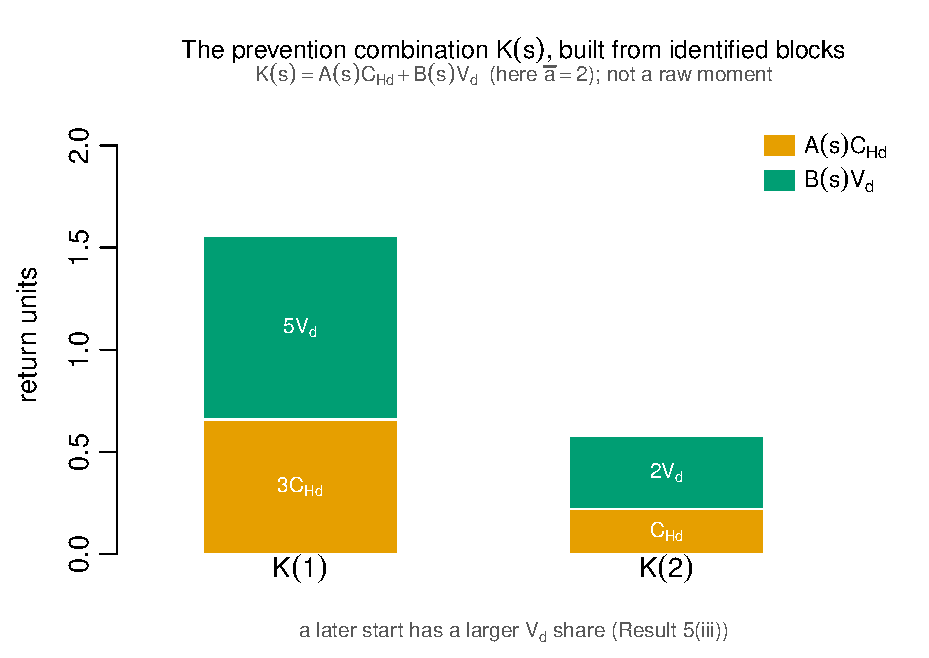
\includegraphics[width = 0.55 \linewidth]{figures/fig_K_bars}
\end{figure}

\subsection*{When the diagonal is not enough}\label{app:props}

\begin{lemma}[When the diagonal is not enough]\label{lem:diag}
(i) With the noise variances $\{v_a\}$ unrestricted, the variance profile $\{\Var(h_a)\}_a$ can never rule out pure noise, nor establish any deterministic heterogeneity: pure noise ($V_H=C_{Hd}=V_d=0$ with $v_a=\Var(h_a)$) reproduces any profile exactly, and so does any $(V_H,C_{Hd},V_d)$ that is a valid second-moment matrix ($V_H,V_d\ge0$, $C_{Hd}^2\le V_HV_d$) and whose implied deterministic variance $V_H+2aC_{Hd}+a^2V_d$ lies weakly below the profile at every observed age.
The diagonal bounds that deterministic variance from above at each age, never from below. (ii) Even with stationary noise variance, the diagonal never separates $V_H$ from the noise: they enter every cell of it only as the bundle $V_H+\sigma^2_u$.
Restoring identification requires stationarity restrictions on the noise for (i), and at least one off-diagonal cell for (ii).
\end{lemma}

\emph{Proof of Lemma~\ref{lem:diag}.} (i) $\Var(h_a)=V_H+2aC_{Hd}+a^2V_d+v_a$.
Given any profile $\{\Var(h_a)\}$, set $V_H=C_{Hd}=V_d=0$ and $v_a=\Var(h_a)\ge0$: the profile is reproduced exactly.
More generally any $(V_H,C_{Hd},V_d)$ with $V_H+2aC_{Hd}+a^2V_d\le\Var(h_a)$ for all observed $a$ is consistent (valid meaning $V_H,V_d\ge0$, $C_{Hd}^2\le V_HV_d$), with $v_a$ the (nonnegative) remainder. (ii) With stationary $\sigma^2_u$, profile differences identify $(C_{Hd},V_d)$, but every diagonal cell is then $(V_H+\sigma^2_u)+\text{known terms}$: shifting $V_H\mapsto V_H+c$, $\sigma^2_u\mapsto\sigma^2_u-c$ leaves the whole diagonal unchanged.
\qed

\subsection*{Proposition~\ref{prop:main}, case by case}

\emph{Case 1 (i.i.d.\ noise, stationary variance).} Any noise with stationary variance gives $\Var(h_a)=V_H+2aC_{Hd}+a^2V_d+\sigma^2_u$, so first differences of the variance profile are $\Var(h_a)-\Var(h_{a-1})=2C_{Hd}+(2a-1)V_d$ and the second difference is $2V_d$ - the reads \eqref{eq:profilereads}.
With $C_{Hd}=0$ the first difference alone is $V_d$ (the benchmark remark).
For the level split, i.i.d.\ noise leaves off-diagonals clean: $\Cov(h_0,h_1)=V_H+C_{Hd}$ gives $V_H$, and $\Var(h_0)=V_H+\sigma^2_u$ gives $\sigma^2_u$.
Overidentification: every remaining cell equals its implied smooth value, e.g.\ $\Cov(h_0,h_2)-\Cov(h_0,h_1)=C_{Hd}$.

\emph{Case 2 (AR(1) noise, stationary variance).} Stationarity gives $\Cov(u_s,u_t)=\sigma^2_u\rho^{\,t-s}$, hence the stated level covariances, and the diagonal reads carry over unchanged (only the stationary marginal variance enters the diagonal).
With $C_{Hd}$ known, the detilted row of the main text, $\tilde C_0(a)=\Cov(h_0,h_a)-aC_{Hd}=V_H+\rho^a\sigma^2_u$ for $a=0,1,2$ (reading $\tilde C_0(0)=\Var(h_0)$), satisfies $\tilde C_0(0)-\tilde C_0(1)=(1-\rho)\sigma^2_u$ and $\tilde C_0(1)-\tilde C_0(2)=\rho(1-\rho)\sigma^2_u$: the ratio is $\rho$, and $\sigma^2_u$, $V_H$ unwind.
$\Cov(h_1,h_2)=V_H+3C_{Hd}+2V_d+\rho\sigma^2_u$ is then implied - the overidentifying check.

\emph{Case 3 (AR(1) noise, age-specific variances).} With $u_a=\rho u_{a-1}+\eta_a$ and free innovation variances, $u_t$ equals $\rho^{\,t-s}u_s$ plus terms independent of $u_s$ (for $t>s$), so $\Cov(u_s,u_t)=\rho^{\,t-s}v_s$ with $v_s\equiv\Var(u_s)$ free.
Row 0 including its diagonal cell satisfies $\Cov(h_0,h_k)=V_H+kC_{Hd}+\rho^k v_0$, so its second differences satisfy
\begin{equation}
S_k\equiv\Cov(h_0,h_{k+1})-2\Cov(h_0,h_k)+\Cov(h_0,h_{k-1})=v_0\rho^{\,k-1}(1-\rho)^2 ,
\end{equation}
where $S_k$ is local shorthand for the second differences written out in \eqref{eq:rowreads3}.
This gives $\rho=S_2/S_1$ with four waves; then $v_0=S_1/(1-\rho)^2$, $V_H=\Var(h_0)-v_0$, and $C_{Hd}=\Cov(h_0,h_1)-\Var(h_0)+(1-\rho)v_0$.
For $V_d$, take the two row-1 cells and eliminate $v_1$:
\begin{equation}
V_d=\frac{\Cov(h_1,h_3)-\rho\,\Cov(h_1,h_2)-(1-\rho)V_H-(4-3\rho)C_{Hd}}{3-2\rho}\,,
\end{equation}
and the remaining $v_a=\Var(h_a)-V_H-2aC_{Hd}-a^2V_d$ come off the diagonals (their off-diagonal counterparts are then overidentifying checks). All verified in \texttt{check\_framework.R}.

\emph{Case 4 (AR(1) noise plus one-period measurement error).} With $u_a=w_a+\varepsilon_a$, $w$ stationary AR(1) and $\varepsilon$ i.i.d., $\Cov(u_s,u_t)=\rho^{\,t-s}\sigma^2_w+\mathbf{1}\{s=t\}\sigma^2_\varepsilon$: the spike adds to every diagonal cell and to no off-diagonal cell.
Total noise variance is constant, so the diagonal reads of Case 1 deliver $(C_{Hd},V_d)$ unchanged.
Detilting the row, $\tilde C_0(a)=V_H+\rho^a\sigma^2_w$ for $a\ge1$ while $\tilde C_0(0)=\Var(h_0)=V_H+\sigma^2_w+\sigma^2_\varepsilon$; successive drops among the off-diagonal cells are $\tilde C_0(a)-\tilde C_0(a+1)=\rho^a(1-\rho)\sigma^2_w$, so their ratio is $\rho$, the scale gives $\sigma^2_w$, the level gives $V_H$, and $\sigma^2_\varepsilon=\Var(h_0)-V_H-\sigma^2_w$ - the reads \eqref{eq:case4reads}.
Three waves are not enough despite the count of six moments for six parameters: given the two diagonal differences, $\Cov(h_1,h_2)-\Cov(h_0,h_1)=2C_{Hd}+2V_d$ is implied, so only three independent equations remain for the four unknowns $(V_H,\rho,\sigma^2_w,\sigma^2_\varepsilon)$ - the map is rank-deficient, and the fourth wave is needed.
Interior cells are then overidentifying checks, e.g.\ $\Cov(h_1,h_2)=V_H+3C_{Hd}+2V_d+\rho\sigma^2_w$.
Applied blind to this world, Case 2's fade read uses the contaminated first drop $\tilde C_0(0)-\tilde C_0(1)=(1-\rho)\sigma^2_w+\sigma^2_\varepsilon$ and understates $\rho$ badly.
The five-wave general member (free $v_s$ and free $\sigma^2_{\varepsilon,s}$) works the same way one row down: second differences of the row \emph{excluding the anchor} give $\rho$ and $v_0$, first differences give $C_{Hd}$, then $V_H$, the spike at each age as the diagonal remainder, and $V_d$ from the interior as in Case 3.
All verified in \texttt{check\_framework.R}, including exact recovery on population moments.

\emph{The denoising case (Appendix~\ref{app:surface}).} With independent noise and free $v_a$, off-diagonal cells are pure smooth layer; along row $a$ the smooth layer is linear in the other index, so its diagonal value is the average of its two neighbours,
\begin{equation}
\tfrac12\bigl[\text{smooth}(a-1,a)+\text{smooth}(a,a+1)\bigr]
=V_H+2aC_{Hd}+a^2V_d=\text{smooth}(a,a),
\end{equation}
which is the interior formula for $\Var^{*}(h_a)$; at the edges extrapolate along row 0 or column 2, e.g.\ $\Var^{*}(h_0)=2\Cov(h_0,h_1)-\Cov(h_0,h_2)$ and $\Var^{*}(h_2)=2\Cov(h_1,h_2)-\Cov(h_0,h_2)$.
The starred profile is the noise-free variance profile, so the Case 1 reads applied to it recover $(V_H,C_{Hd},V_d)$, and $v_a=\Var(h_a)-\Var^{*}(h_a)$.
Expanding the starred formulas reproduces the covariance-only solve ($C_{Hd}=\Cov(h_0,h_2)-\Cov(h_0,h_1)$, etc.) term by term.

\subsection*{The $D_k$ ladder}

The ladder is a diagnostic rather than a step in any proof: it reads the noise process off changes instead of levels. With $\gamma(k)=\sigma^2_u\rho^k$,
\begin{equation}
\Cov(\Delta u_t,\Delta u_{t+k})=2\gamma(k)-\gamma(k-1)-\gamma(k+1)
=-\sigma^2_u(1-\rho)^2\rho^{\,k-1}, \qquad k\ge1,
\end{equation}
so $D_k=V_d-(1-\rho)^2\rho^{\,k-1}\sigma^2_u$: dip-then-flat at $\rho=0$, a geometric rise for $\rho\in(0,1)$, flat at $\rho=1$.
Note that dip-then-flat is shared by the random-walk-plus-spike class of Proposition~\ref{prop:F1} ($D_1=V_d-\sigma^2_\varepsilon$, $D_k=V_d$ for $k\ge2$), so the ladder alone does not separate i.i.d.\ noise from that class - the level staircase does.
Successive gaps give $\rho=(D_3-D_2)/(D_2-D_1)$ (five waves).
An added i.i.d.\ spike $\varepsilon$ changes no $D_k$ with $k\ge2$ (adjacent changes alone share an $\varepsilon$) but shifts $D_1$ by $-\sigma^2_\varepsilon$, so the five-wave formula is not spike-robust either: the spike-robust recovery uses gaps among the $k\ge2$ rungs only, $\rho=(D_4-D_3)/(D_3-D_2)$, at the cost of a sixth wave.
The three-wave fade solve fails under a spike for the same reason (the spike enters the detilted row at $a=0$ but none of its off-diagonal cells); Case 4 is the level-based repair, moving the fade read to drops the spike cannot touch at the cost of a fourth wave.
The simulation check in \texttt{check\_framework.R} ($N=2\times10^6$) recovers all parameters to two-three decimals under both spike-free routes.

\section{The value of targeting: pricing information sets}\label{sec:targeting}\label{app:target}

This appendix proves the targeting results of Section~\ref{sec:target0} and adds the comparison between type- and level-targeting.
Throughout, $\mu(z)$ is an allocation rule based on information $z$, with average intensity held fixed at $\E[\mu(z)]=\bar\mu$.

\begin{itemize}
\item Result~\ref{res:collect} is the accounting identity: any rule saves exactly $\Cov\bigl(\mu(z),\E[P_i\mid z]\bigr)$ over the uniform policy.
The optimality counterpart is Lemma~\ref{lem:info}: per unit of intensity dispersion, no rule based on $z$ beats $\mathrm{sd}\bigl(\E[P_i\mid z]\bigr)$.
\item Result~\ref{res:type}'s third-moment point, formally: $P_j(r)=2\sum_{a\ge r}(1-H_j-a\,d_j)\bigl(-(a-r+1)d_j\bigr)$ is quadratic in $(H_j,d_j)$, so the spread of $P_j$ across types - the object any type-based scheme collects - involves third and fourth moments of the type distribution, beyond the covariance surface of Section~\ref{sec:ident}.
This is the sense in which targeting is priced by the type distribution (clusters), not by second moments.
\end{itemize}

\begin{lemma}[Value of an information set]\label{lem:info}
To first order in intensities, the saving of allocation $\mu(z)$ over the uniform policy with the same average intensity is $\Cov\bigl(\mu(z),\E[P_i\mid z]\bigr)$ (Result~\ref{res:collect}).
Per unit of intensity dispersion $\mathrm{sd}(\mu)$, no rule based on $z$ can save more than $\mathrm{sd}\bigl(\E[P_i\mid z]\bigr)$, with equality when $\mu$ is increasing and affine in $\E[P_i\mid z]$.
An information set is worth the return dispersion it reveals. (proof below.)
\end{lemma}

%\begin{remark}[Dispersion cap vs.\ box constraints]
%Imposing $\mu\in[0,1]$ instead of the dispersion cap also yields a well-posed problem; the optimum is then bang-bang - full intensity for the top-$\bar\mu$ quantile of predicted returns $\E[P_i\mid z]$, zero for the rest - with gain $\bar\mu\,(\E[P_i\mid \text{top }\bar\mu]-\E[P_i])$, an upper-tail object that depends on the whole distribution of $\E[P_i\mid z]$, not just second moments. If $\E[P_i\mid z]$ is Gaussian, this equals $\varphi(\Phi^{-1}(1-\bar\mu))\cdot\mathrm{sd}(\E[P_i\mid z])$: proportional to the same dispersion, with a budget-only factor common to every information set, so all rankings and ratios below are unchanged. The dispersion cap delivers this proportionality distribution-free and keeps the value of information in the same second-moment currency as the identification results of Section~\ref{sec:ident}. Its linear rule can in principle leave $[0,1]$: with finitely many types (bounded returns) it stays inside exactly for $\kappa$ small enough, while for unbounded signals clipping to $[0,1]$ is required on a tail event whose cost vanishes faster than $\kappa$ - so the $\kappa\,\mathrm{sd}$ formula is exact for type-targeting and leading-order otherwise (derivations below).
%\end{remark}

\begin{result}[Targeted vs.\ uniform prevention; $z=$ type]\label{res:T1}
Bound for Result~\ref{res:type}: the saving from any type-based allocation is $\Cov_j\bigl(\mu_j,P_j(r)\bigr)\le\mathrm{sd}(\mu)\,\mathrm{sd}_j\bigl(P_j(r)\bigr)$; it is zero iff $P_j(r)$ is constant across types.
The opportunity cost of \emph{not} targeting is the foregone covariance.
\end{result}

\begin{result}[Type- vs.\ level-targeting; $z=h_{i,r-1}$]\label{res:T2}
Let the level signal be the last pre-intervention observation $h_{i,r-1}$. If $u$ is i.i.d., future gaps depend on $z$ only through the type, so $\E[P_i\mid h_{i,r-1}]=\E[P_j\mid h_{i,r-1}]$ and
\begin{equation}
\frac{\text{gain from level-targeting}}{\text{gain from type-targeting}}
=\frac{\mathrm{sd}\bigl(\E[P_j\mid h_{i,r-1}]\bigr)}{\mathrm{sd}_j\bigl(P_j\bigr)}\;\le\;1,
\qquad
\text{(linear rules: } \bigl|\Corr(h_{i,r-1},P_j)\bigr| \text{)}.
\end{equation}
\end{result}

\begin{itemize}
\item Two forces keep the ratio below one: (i) \emph{span} - a single level reveals only one combination, $H+(r-1)d$ plus noise, of the two traits $(H,d)$ that drive $P_j$; (ii) \emph{attenuation} - $v_{r-1}$ in $\Var(h_{r-1})$ shrinks the projection.
The value of clustering is the residual dispersion, largest when current level poorly predicts subsequent decline - and directly computable once clusters are estimated (compute $P_j$ per cluster, project on the pre-period level).
\item In the linear case the two forces factor cleanly: writing $h_{i,r-1}=\bar h_{i,r-1}+u_{i,r-1}$, where $\bar h_{i,r-1}=H_i+(r-1)d_i$ is the individual's expected (deterministic) health,
\begin{equation}
\begin{gathered}
\Corr(h_{r-1},P_j)=\sqrt{\lambda_{r-1}}\;\Corr(\bar h_{i,r-1},P_j),
\\
\lambda_{r-1}\equiv\frac{\Var(\bar h_{i,r-1})}{\Var(h_{r-1})}
=\frac{V_H+2(r-1)C_{Hd}+(r-1)^2V_d}{V_H+2(r-1)C_{Hd}+(r-1)^2V_d+v_{r-1}}\,,
\end{gathered}
\end{equation}
a signal-reliability factor $\sqrt{\lambda_{r-1}}$ (attenuation, computable from Proposition~\ref{prop:main}) times a span factor $\Corr(\bar h_{i,r-1},P_j)$ (generically $<1$: one linear combination of two traits).
\item If $u$ is persistent (random walk), level-targeting gains a genuine extra role: deviations persist into future levels and raise individual returns through the gap term.
If $u$ is mean-reverting, levels \emph{mislead}: dips predict recovery.
Both cases reinforce that the deterministic component is the reliable targeting object.
\end{itemize}

Notation for the proofs: $\mathcal{C}_i$ is individual $i$'s lifetime cost (Section~\ref{sec:cost}), $P_i$ their marginal return to prevention (the reduction in expected lifetime cost per unit of intensity), and $z_i$ the information the allocation may condition on; the predicted return is written $\E[P_i\mid z]$ throughout.

\subsection*{Proof of Lemma~\ref{lem:info}}

\emph{Step 1: linearize in intensities.} Giving individual $i$ intensity $\mu_i$ lowers their expected cost by $\mu_i P_i$ to first order (that is the definition of the marginal return) so for any allocation rule $\mu(\cdot)$,
\begin{equation}
\E[\mathcal{C}_i(\mu(\cdot))]\;=\;\E[\mathcal{C}_i(0)]-\E[\mu(z_i)\,P_i]+O(\mu^2).
\end{equation}

\emph{Step 2: only the predicted return matters.} The rule can respond to $z_i$ only, so by the law of iterated expectations,
\begin{equation}
\E[\mu(z_i)\,P_i]\;=\;\E\bigl[\mu(z_i)\,\E(P_i\mid z_i)\bigr].
\end{equation}

\emph{Step 3: split the effect into budget and targeting.}
\begin{equation}
\E\bigl[\mu(z)\,\E[P_i\mid z]\bigr]
\;=\;
\underbrace{\bar\mu\,\E[P_i]}_{\text{uniform policy, same budget}}
\;+\;
\underbrace{\Cov\bigl(\mu(z),\E[P_i\mid z]\bigr)}_{\text{gain from targeting}} ,
\end{equation}
so the cost reduction of $\mu(z)$ over uniform $\bar\mu$ is exactly the covariance, as stated in the lemma.

\emph{Step 4: the bound.} By Cauchy-Schwarz, $\Cov(\mu,\E[P_i\mid z])\le\mathrm{sd}(\mu)\,\mathrm{sd}(\E[P_i\mid z])$, with equality iff $\mu$ is an increasing affine transform of $\E[P_i\mid z]$:
\begin{equation}
\mu^*(z)\;=\;\bar\mu+\mathrm{sd}(\mu)\,\frac{\E[P_i\mid z]-\E[P_i]}{\mathrm{sd}(\E[P_i\mid z])},
\qquad
\text{saving}\;=\;\mathrm{sd}(\mu)\,\mathrm{sd}\bigl(\E[P_i\mid z]\bigr).
\end{equation}

\subsection*{Feasibility of the linear rule}

The rule $\mu^*(z)$ stays in $[0,1]$ for every $z$ iff
\begin{equation}
\mathrm{sd}(\mu)\;\le\;\min(\bar\mu,\,1-\bar\mu)\;\frac{\mathrm{sd}(\E[P_i\mid z])}{\max_z\,\bigl|\E[P_i\mid z]-\E[P_i]\bigr|},
\end{equation}
which holds automatically for small $\mathrm{sd}(\mu)$ whenever returns are bounded - in particular for finitely many types, so Result~\ref{res:T1} needs no caveat.
When $\E[P_i\mid z]$ is unbounded (e.g.\ a Gaussian level signal), clip the rule to $[0,1]$.
Writing $S=(\E[P_i\mid z]-\E[P_i])/\mathrm{sd}(\E[P_i\mid z])$, clipping binds only on the tail event $|S|>\min(\bar\mu,1-\bar\mu)/\mathrm{sd}(\mu)$ and forgoes saving $\mathrm{sd}(\mu)\,\mathrm{sd}(\E[P_i\mid z])\,\E\bigl[S^2;\,|S|>\min(\bar\mu,1-\bar\mu)/\mathrm{sd}(\mu)\bigr]$ - exponentially small in $1/\mathrm{sd}(\mu)$ for Gaussian signals - so the stated saving is exact to leading order.

\subsection*{Alternative: box constraints and bang-bang targeting}

Impose $\mu(z)\in[0,1]$ instead of fixing the dispersion of $\mu$, keeping the budget $\E[\mu]=\bar\mu$.
The objective is linear in $\mu(z)$ pointwise, so the optimum is a corner solution: $\mu=1$ where $\E[P_i\mid z]$ exceeds a threshold and $\mu=0$ below it, with the threshold set so the treated group has mass $\bar\mu$ - ``treat the top $\bar\mu$ quantile''.
The gain over uniform is the upper-tail object
\begin{equation}
\bar\mu\,\bigl(\E[P_i\mid\text{top }\bar\mu]-\E[P_i]\bigr).
\end{equation}
If $\E[P_i\mid z]$ is Gaussian, the truncated-normal mean $\E[P_i\mid\text{top }q]=\E[P_i]+\mathrm{sd}(\E[P_i\mid z])\,\varphi(\Phi^{-1}(1-q))/q$ turns this into $\varphi(\Phi^{-1}(1-\bar\mu))\,\mathrm{sd}(\E[P_i\mid z])$: proportional to the same dispersion, with a factor that depends only on the budget - hence identical comparisons across information sets as under the affine rule.

\paragraph{Remark (budget devices).} Fixing the dispersion of $\mu$ leads to an affine
rule; the box constraint leads to treating the top-$\bar\mu$ quantile.
Either way the saving is a budget factor, common to every information set, times $\mathrm{sd}\bigl(\E[P_i\mid z]\bigr)$ (for the box case, exactly so under Gaussian signals).
Nothing in the text depends on which device is used: every comparison in Results~\ref{res:T1}-\ref{res:T2} and Result~\ref{res:target} is a ratio or a difference in which the budget factor cancels.

\subsection*{Proof of Result~\ref{res:T2}}

The level signal is the last pre-intervention observation $h_{i,r-1}$, and $u$ is i.i.d.

\emph{Step 1: the level signal predicts returns only through the type.} For $a\ge r$, $\Cov(u_{r-1},u_a)=0$, so conditional on $(j,h_{r-1})$ the expected future gaps equal the type gaps $1-\bar h_{j,a}$.
Hence $P_i=P_j$, and $\E[P_i\mid h_{r-1}]=\E[P_j\mid h_{r-1}]$.

\emph{Step 2: apply the lemma to each information set.} Per unit of intensity dispersion, type-targeting saves $\mathrm{sd}_j(P_j)$; level-targeting saves $\mathrm{sd}\bigl(\E[P_j\mid h_{r-1}]\bigr)$.

\emph{Step 3: the ratio is below one.} Conditioning can only shrink variance (law of total variance): $\Var\bigl(\E[P_j\mid h_{r-1}]\bigr)\le\Var_j(P_j)$, giving the stated ratio.

\emph{Step 4: linear rules give the correlation form.} For $\mu=\bar\mu+b\,h_{r-1}$,
\begin{equation}
\frac{\text{saving}}{\text{intensity dispersion}}
=\frac{b\,\Cov(h_{r-1},P_j)}{|b|\,\mathrm{sd}(h_{r-1})}
=\pm\,\Corr(h_{r-1},P_j)\,\mathrm{sd}(P_j),
\end{equation}
so the best linear rule saves $|\Corr(h_{r-1},P_j)|\,\mathrm{sd}(P_j)$ per unit of dispersion.

\emph{Step 5: reliability factorization (as used in the discussion of Result~\ref{res:T2}).} Since $u_{r-1}$ is uncorrelated with $(H_i,d_i)$ and $P_j$ is a function of them, $\Cov(h_{r-1},P_j)=\Cov(\bar h_{i,r-1},P_j)$ while $\Var(h_{r-1})=\Var(\bar h_{i,r-1})+v_{r-1}$.
Hence $\Corr(h_{r-1},P_j)=\sqrt{\lambda_{r-1}}\,\Corr(\bar h_{i,r-1},P_j)$ with $\lambda_{r-1}=\Var(\bar h_{i,r-1})/\Var(h_{r-1})$.

\subsection*{Proof of Results~\ref{res:target} and~\ref{res:type}}

Write $C_0\equiv\Cov\bigl(h_{i,0},P_i(r)\bigr)$ for the covariance in Result~\ref{res:target}.

\emph{Step 1: noise in the signal drops out.} $P_i=P_{j(i)}$ is a function of the type alone (Result~\ref{res:prevj}) and $\E[u_{i,0}\mid j]=0$, so $\Cov(u_{i,0},P_i)=\E\bigl[P_j\,\E[u_{i,0}\mid j]\bigr]=0$ and $C_0=\Cov_j(\bar h_{j,0},P_j)$.
Likewise $\Var(h_{i,0})=\Var_j(\bar h_{j,0})+v_0$ with $v_0\equiv\E_j\bigl[\Var(u_{i,0}\mid j)\bigr]$.

\emph{Step 2: the projection slope.} By definition $\beta(r)=\Cov(h_{i,0},P_i)/\Var(h_{i,0})$, which with Step 1 is \eqref{eq:beta0}.

\emph{Step 3: the two channels.} At each age $P_j$ pairs the gap $Y_a\equiv1-\bar h_{j,a}$ with the preventable decline $Z_a\equiv\bar h_{j,r-1}-\bar h_{j,a}$.
For any three variables, $\Cov(X,YZ)=\E[Y]\Cov(X,Z)+\E[Z]\Cov(X,Y)+\E[\tilde X\tilde Y\tilde Z]$ with tildes denoting deviations from means.
Apply this with $X=\bar h_{j,0}$: the means are $\E_j[Y_a]=1-\bar h_a$ and $\E_j[Z_a]=\bar h_{r-1}-\bar h_a$, and $\Cov_j(\bar h_{j,0},Y_a)=-\Cov_j(\bar h_{j,0},\bar h_{j,a})$.
Summing over $a\ge r$ and dropping the third central moments gives \eqref{eq:G0}.

\emph{Step 4: the linear case.} With $\bar h_{j,a}=H_j+a\,d_j$ we have $\Cov_j(\bar h_{j,0},\bar h_{j,a})=V_H+aC_{Hd}$ and $Z_a=-(a-r+1)d_j$, so $\Cov_j(\bar h_{j,0},Z_a)=-(a-r+1)C_{Hd}$; substituting into \eqref{eq:G0} and collecting the exposure weight $(a-r+1)$ gives \eqref{eq:G0lin}.
Carrying out the sums with $A(r)$, $B(r)$ of \eqref{eq:Ks} gives the equivalent closed form $2A(r)\bar d\,V_H+2C_{Hd}\bigl[A(r)(\bar H-1)+2B(r)\bar d\bigr]$.

\emph{Step 5: per-person comparisons.} A person one standard deviation below the mean has predicted return $\E[P_i]-\beta(r)\,\mathrm{sd}(h_0)$, which under $\beta(r)<0$ lies $|\beta(r)|\,\mathrm{sd}(h_0)$ above the mean.
Moving one unit of intensity from a person one sd above to one one sd below changes cost by the difference in their predicted returns, $2|\beta(r)|\,\mathrm{sd}(h_0)$ (Result~\ref{res:collect}), leaving average intensity unchanged.

\emph{Step 6: attenuation.} If the type's own level $\bar h_{j,0}$ were observed, the projection of $P_i$ on it would have slope $C_0/\Var_j(\bar h_{j,0})$ - same covariance, smaller variance - so $\beta(r)$ is that slope times $\lambda_0=\Var_j(\bar h_{j,0})/\bigl(\Var_j(\bar h_{j,0})+v_0\bigr)$.
The per-sd comparison scales with $|C_0|/\mathrm{sd}(\cdot)$ and $\mathrm{sd}_j(\bar h_{j,0})/\mathrm{sd}(h_0)=\sqrt{\lambda_0}$, giving the $\sqrt{\lambda_0}$ factor.

\emph{Step 7: the ceiling (Result~\ref{res:type}).} The per-person statements are Result~\ref{res:collect} with $z$ the type.
For the ceiling, $\E[P_i\mid z] =\E\bigl[\E[P_i\mid j]\mid z\bigr]=\E[P_j\mid z]$, so by the law of total variance $\Var\bigl(\E[P_j\mid z]\bigr)\le\Var_j(P_j)$, with equality iff $z$ determines $P_j$.
\qed

\section{Growth-regression representation: equivalence and corrections}\label{app:growth}

Every case of Proposition~\ref{prop:main} can equivalently be expressed in terms of individual growth regressions: OLS of $h_{i,a}$ on $(1,a)$, keeping intercepts $\hat H_i$, slopes $\hat d_i$ and residuals $e_i$.
Three things are worth separating.

\begin{itemize}
\item The representation is general.
Writing $(\hat H_i,\hat d_i,e_i)=M h_i$, the matrix $M$ depends only on which waves are used, not on the noise process, and is invertible; the coefficient second moments are therefore the congruence $M\,\Var(h)\,M'$ of the level covariance matrix, whatever the noise.
The two coordinate systems always carry identical information.
\item The dictionary is case-specific.
With $\hat\theta_i=\theta_i+Au_i$ and $e_i=Ru_i$, the noise enters as $A\Sigma_uA'$, $A\Sigma_uR'$ and $R\Sigma_uR'$.
Under i.i.d.\ noise these collapse to $\sigma^2_u(X'X)^{-1}$ and $\sigma^2_uRR'$, giving the dictionary below.
Under memory they involve $\rho$ as well, and under age-specific variances the design weights the individual $v_a$: the corrections change, the transform does not.
\item Numerical equivalence needs just-identification.
When both routes solve the same just-identified system they return identical estimates in any sample.
With overidentifying moments and a fixed weight matrix, the two routes agree only if the weighting is mapped through the same transform.
\end{itemize}

Two practical caveats.
The design must match the deterministic basis, so if a quadratic age term is added (Section~\ref{sec:linear}) the regression becomes OLS on $(1,a,a^2)$ and the same argument goes through with three coefficients.
Residual coordinates exist only from three waves on; with two waves the regression fits exactly and the noise correction must come from an off-diagonal cell.
This is also why the empirical-Bayes shortcut at the end of this appendix fails under memory: the failure is in the noise correction, not in the representation.
The congruence is verified under all three noise processes in \texttt{check\_framework.R}.

\subsection*{Equivalence}
Fix waves $a=0,\dots,T-1$ and the design $X=[\mathbf{1},a]$.
Individual OLS gives $(\hat H_i,\hat d_i)'=(X'X)^{-1}X'h_i$; let $e_i$ collect the residual coordinates (any basis of the orthogonal complement of $\mathrm{col}(X)$, dimension $T-2$).
Then $(\hat H_i,\hat d_i,e_i)=M h_i$ with $M$ invertible, so the second-moment matrix of $(\hat H,\hat d,e)$ is the congruence $M\,\Var(h)\,M'$ of the level covariance matrix: the two coordinate systems carry \emph{identical} information.
Moreover the model's moment equations are \emph{linear} in $(V_H,V_d,C_{Hd},v_a)$ and, with three waves, just-identified with a unique solution; hence any valid solving route - level moments (the denoising solve of Appendix~\ref{app:surface}) or coefficient moments (below) - returns \emph{numerically identical} estimates in any sample.
The two-wave benchmark ($C_{Hd}=0$) is the special case where the regression fits exactly, $\hat H_i=h_{i,0}$ and $\hat d_i=\Delta h_{i,1}$, and the noise correction comes from $\Cov(h_0,h_1)$.

\subsection*{Three-wave dictionary (Case 1: i.i.d.\ noise)}
With $a=0,1,2$:
\begin{equation}
\hat d_i=\tfrac{h_{i,2}-h_{i,0}}{2}=d_i+\tfrac{u_{i,2}-u_{i,0}}{2},
\qquad
\hat H_i=\tfrac{5h_{i,0}+2h_{i,1}-h_{i,2}}{6}=H_i+\tfrac{5u_{i,0}+2u_{i,1}-u_{i,2}}{6},
\end{equation}
\begin{equation}
e_i=h_{i,0}-2h_{i,1}+h_{i,2}=u_{i,0}-2u_{i,1}+u_{i,2}
\quad\text{(the deterministic part is annihilated exactly)}.
\end{equation}
Second moments:
\begin{align}
\Var(\hat d)&=V_d+\tfrac{v_0+v_2}{4}, &
\Cov(\hat H,\hat d)&=C_{Hd}-\tfrac{5v_0+v_2}{12}, &
\Var(\hat H)&=V_H+\tfrac{25v_0+4v_1+v_2}{36},\\
\Var(e)&=v_0+4v_1+v_2, &
\Cov(\hat d,e)&=\tfrac{v_2-v_0}{2}, &
\Cov(\hat H,e)&=\tfrac{5v_0-4v_1-v_2}{6}.
\end{align}
The residual block (second row) identifies $(v_0,v_1,v_2)$; substituting into the first row corrects $\Var(\hat d)$ and $\Cov(\hat H,\hat d)$ and reproduces the denoising solve of Appendix~\ref{app:surface} exactly.

\emph{Interpretation.} The first row is where the regression version earns its keep: $V_d$ is \emph{observed slope dispersion minus estimation noise} (the empirical-Bayes/shrinkage correction of the value-added and firm-effects literatures), and $C_{Hd}$ is the intercept-slope covariance purged of the \emph{mechanical negative correlation} from shared noise (a low baseline draw lowers $\hat H_i$ and raises $\hat d_i$).

\subsection*{The EB shortcut and its biases}
EB $=$ empirical Bayes: since estimated slopes are noisy, their raw dispersion overstates $V_d$ by the average squared standard error, so the textbook practice (as in the teacher value-added and firm-effects literatures) subtracts it - the variance-estimation step of an empirical-Bayes shrinkage procedure.
Concretely, the shortcut estimates $\hat\sigma^2_i=e_i^2/6$ (RSS over $T-2=1$ d.f.), $\widehat{SE}(\hat d_i)^2=\hat\sigma^2_i/2$, and corrects $\widehat{V}^{\,EB}_d=\Var(\hat d_i)-\E[\hat\sigma^2_i]/2$.
This replaces the three residual-block equations with one pooled homoskedastic equation, and is \emph{not} the same statistic:
\begin{itemize}
\item i.i.d.\ noise, age-varying variance: bias $=\tfrac{v_0-2v_1+v_2}{6}$ (zero iff $v_a$ is linear in age; can push the estimate negative);
\item random walk $+$ i.i.d.\ noise (constant variances): bias $=+\sigma^2_\eta/3$ - permanent innovations masquerade as slope heterogeneity (the HIP/RIP confound).
\end{itemize}

\subsection*{Simulation check}
$N=2\times10^6$, four waves, true $V_d=0.040$, $C_{Hd}=0.050$ (\texttt{check\_framework.R}):
\begin{center}
\small
\begin{tabular}{@{}lccccc@{}}
\toprule
& \multicolumn{4}{c}{$\hat V_d$ (true $0.040$)} & $\hat C_{Hd}$ (true $0.050$)\\
\cmidrule(lr){2-5}\cmidrule(l){6-6}
Noise scenario & denoise & growth-reg. & EB shortcut & Prop.~\ref{prop:F1} & denoise $=$ g-reg.\\
\midrule
i.i.d., homoskedastic            & 0.0401 & 0.0401 & 0.0402    & 0.0399 & 0.0503\\
i.i.d., age-varying $v_a$ & 0.0421 & 0.0421 & $-$0.0250 & 0.0389 & 0.0484\\
random walk $+$ noise            & 0.1406 & 0.1406 & 0.1065    & 0.0389 & 0.0487\\
\bottomrule
\end{tabular}
\end{center}
The denoising solve and its growth-regression twin agree to $\le4\times10^{-14}$ in every scenario - including the third, where both are biased \emph{identically} (the same statistic in different coordinates).
The EB biases match the formulas above ($0.040-0.067=-0.027$; $0.040+0.067=0.107$), and the denoising solve's random-walk bias is $+\sigma^2_\eta/2=0.100$, from $\Cov(h_1,h_2)$ absorbing $\sigma^2_{\eta,1}$.
With $T>3$ waves both systems are overidentified in the same way (the bijection preserves the moment count); the lag-moment combinations of Case 2 and Proposition~\ref{prop:F1} remain natural ones for serial dependence.

\section{The general covariance surface}\label{app:surface}

The cases of Proposition~\ref{prop:main} are cells of one template, stated fully generally in \eqref{eq:template}.
One noise class deserves its own display - ``random walk ($\eta$, initial variance $\omega^2$) $+$ i.i.d.\ ($\varepsilon$)'', the class of Proposition~\ref{prop:F1} below (the $\rho\to1$ member of the Case 3 family \eqref{eq:case3noise} with a spike added) - for which every second moment of the panel is one equation:
\begin{equation}
\Cov(h_s,h_t)
\;=\;
\underbrace{B}_{\text{level}}
\;+\;
\underbrace{(s+t)\,C_{Hd}}_{\text{tilt}}
\;+\;
\underbrace{st\,V_d}_{\text{curvature}}
\;+\;
\underbrace{G(\min(s,t))}_{\text{staircase}}
\;+\;
\underbrace{\mathbf{1}\{s=t\}\,\sigma^2_{\varepsilon,s}}_{\text{diagonal spike}},
\label{eq:surface}
\end{equation}
with $B\equiv V_H+\omega^2$ and $G(m)\equiv\sum_{\ell\le m}\sigma^2_{\eta,\ell}$, $G(0)=0$; and fully generally, for any deterministic basis $f_1,\dots,f_K$ and any noise process,
\begin{equation}
\Cov(h_s,h_t)\;=\;\sum_{k,l}\Omega_{kl}\,f_k(s)f_l(t)\;+\;\gamma_u(s,t),
\label{eq:template}
\end{equation}
where $\Omega$ is the second-moment matrix of the deterministic traits and $\gamma_u$ the noise autocovariance.
Our linear case is $f=(1,a)$; Case 2 is $\gamma_u(s,t)=\sigma^2_u\rho^{\,t-s}$; Case 3 is $\gamma_u(s,t)=\rho^{\,t-s}v_s$ (Figure~\ref{fig:menu} shows the menu of layers).

\begin{figure}[H]
	\centering
	\caption{The covariance matrix, layer by layer (colours as in the anatomy charts)}
	\label{fig:layers}
	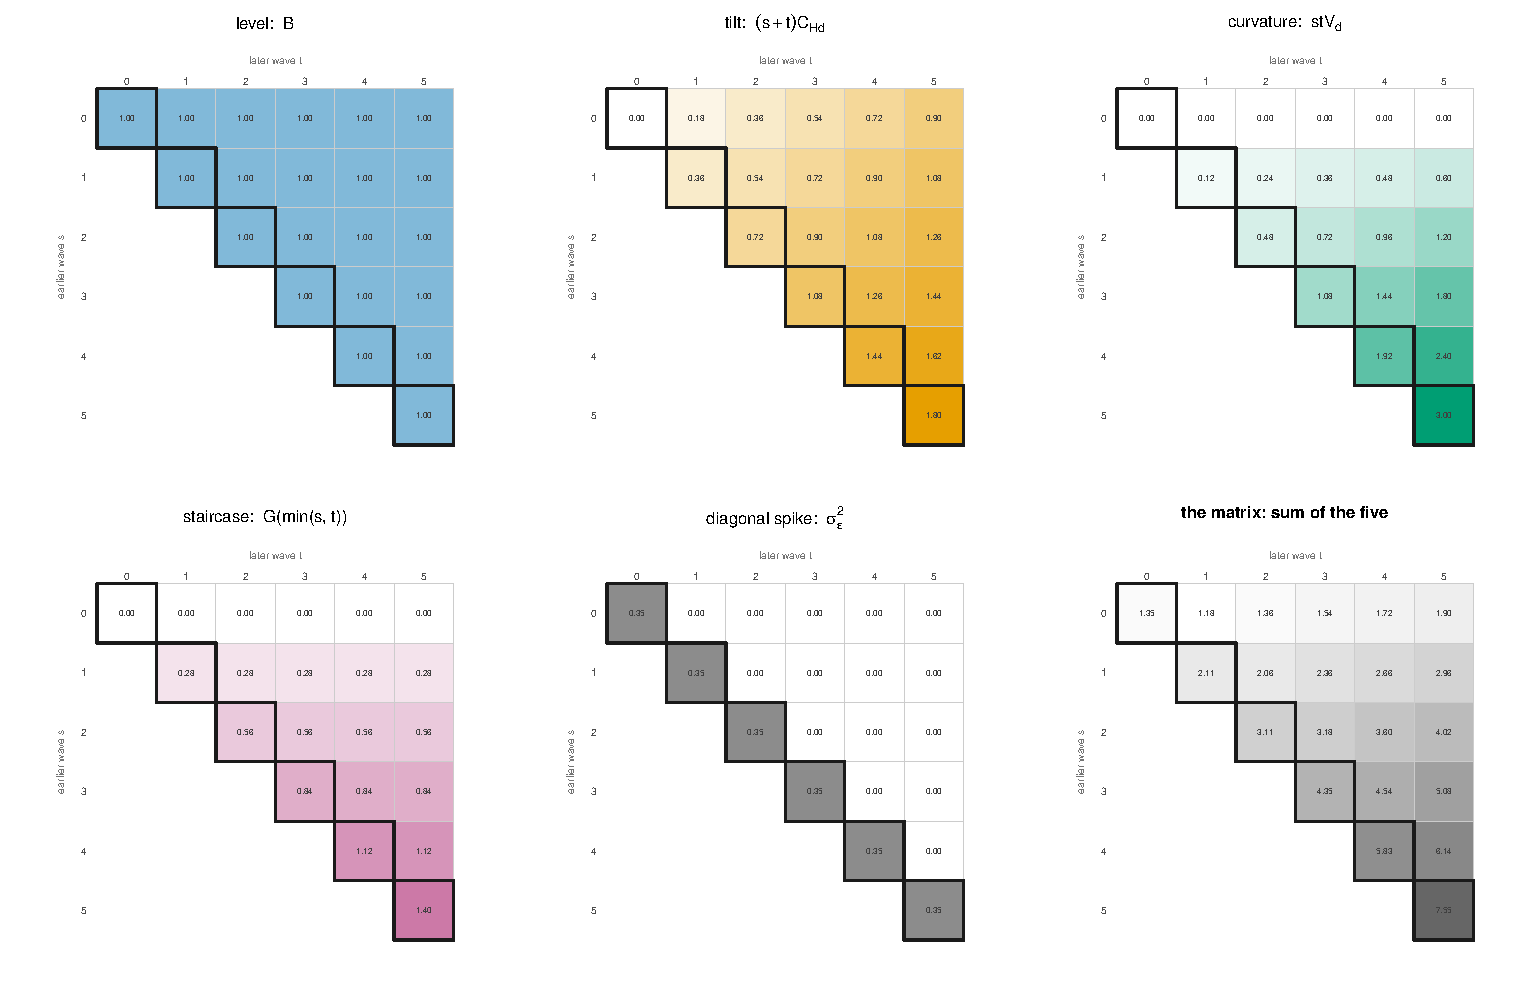
\includegraphics[width=\textwidth]{figures/fig_surface_layers_tri}
\end{figure}

\begin{itemize}
\item Where the terms come from (Figure~\ref{fig:layers}): the deterministic part contributes the polynomial layers, because $(H_i+s\,d_i)(H_i+t\,d_i)=H_i^2+(s+t)H_id_i+st\,d_i^2$ - the product of two trend lines, multiplied out.
The noise contributes the local layers: the walk shared up to the earlier wave ($\min(s,t)$), and the i.i.d.\ part only where a wave meets itself.
\item The triad of Section~\ref{sec:triad} maps onto the layers: \emph{stays} $=$ level $+$ staircase, \emph{the moment} $=$ the spike, \emph{evolving} $=$ tilt $+$ curvature.
The forces that keep these apart are in Section~\ref{sec:forces}; the boundary case is a ``noise'' whose autocovariance were proportional to $st$, which would be an individual drift, i.e.\ it \emph{is} a deterministic slope.
\end{itemize}

\subsection*{Vocabulary}

\begin{center}
\small
\begin{tabular}{@{}p{2.6cm}p{5.2cm}p{5.6cm}@{}}
\toprule
\textbf{Term here} & \textbf{Meaning on the matrix} & \textbf{Standard counterpart} \\
\midrule
surface & $\Cov(h_s,h_t)$ as height over $(s,t)$ & ``covariance structure'' (earnings
dynamics); ``covariance function/surface'' (functional data analysis) \\
level $B$ & constant height everywhere & fixed-effect variance ($\sigma^2_\alpha$), bundled
with initial permanent variance \\
tilt $(s+t)C_{Hd}$ & plane sloping up toward late-late pairs & intercept-slope covariance
$\sigma_{\alpha\beta}$ in HIP earnings models \\
curvature $st\,V_d$ & twist of the surface: the cross-derivative
$\partial^2/\partial s\,\partial t$ & slope variance $\sigma^2_\beta$; ``heterogeneous
profiles'' \\
staircase $G(\min(s,t))$ & terraces rising toward the diagonal & the unit-root signature:
covariances growing in $\min(s,t)$ (the unit-root literature; see the companion note) \\
diagonal spike $\sigma^2_\varepsilon$ & a ridge only where $r=t$ & measurement error; the
``nugget effect'' in geostatistics \\
\bottomrule
\end{tabular}
\end{center}

\begin{itemize}
\item The spike is not an extra ingredient: it is the i.i.d.\ component already in the main text - the entire noise in Case 1.
Whether it is measurement error or genuine transitory health variation cannot be distinguished from second moments (both paint only the diagonal), but the interpretation matters for welfare: measurement error should be \emph{excluded} from $\Var(h_a)$ in the treatment return $T(r)$, while the prevention return $P(r)$ never contains the spike and so is immune to the question - the caveat in Section~\ref{sec:compare}.
\item The earnings-dynamics ancestry of every object here, with full references, is documented in the companion note \texttt{earnings\_comparison\_note.tex}.
\end{itemize}

\begin{figure}[H]
	\centering
	\caption{The general template as a menu: pick one smooth layer, add noise layers}
	\label{fig:menu}
	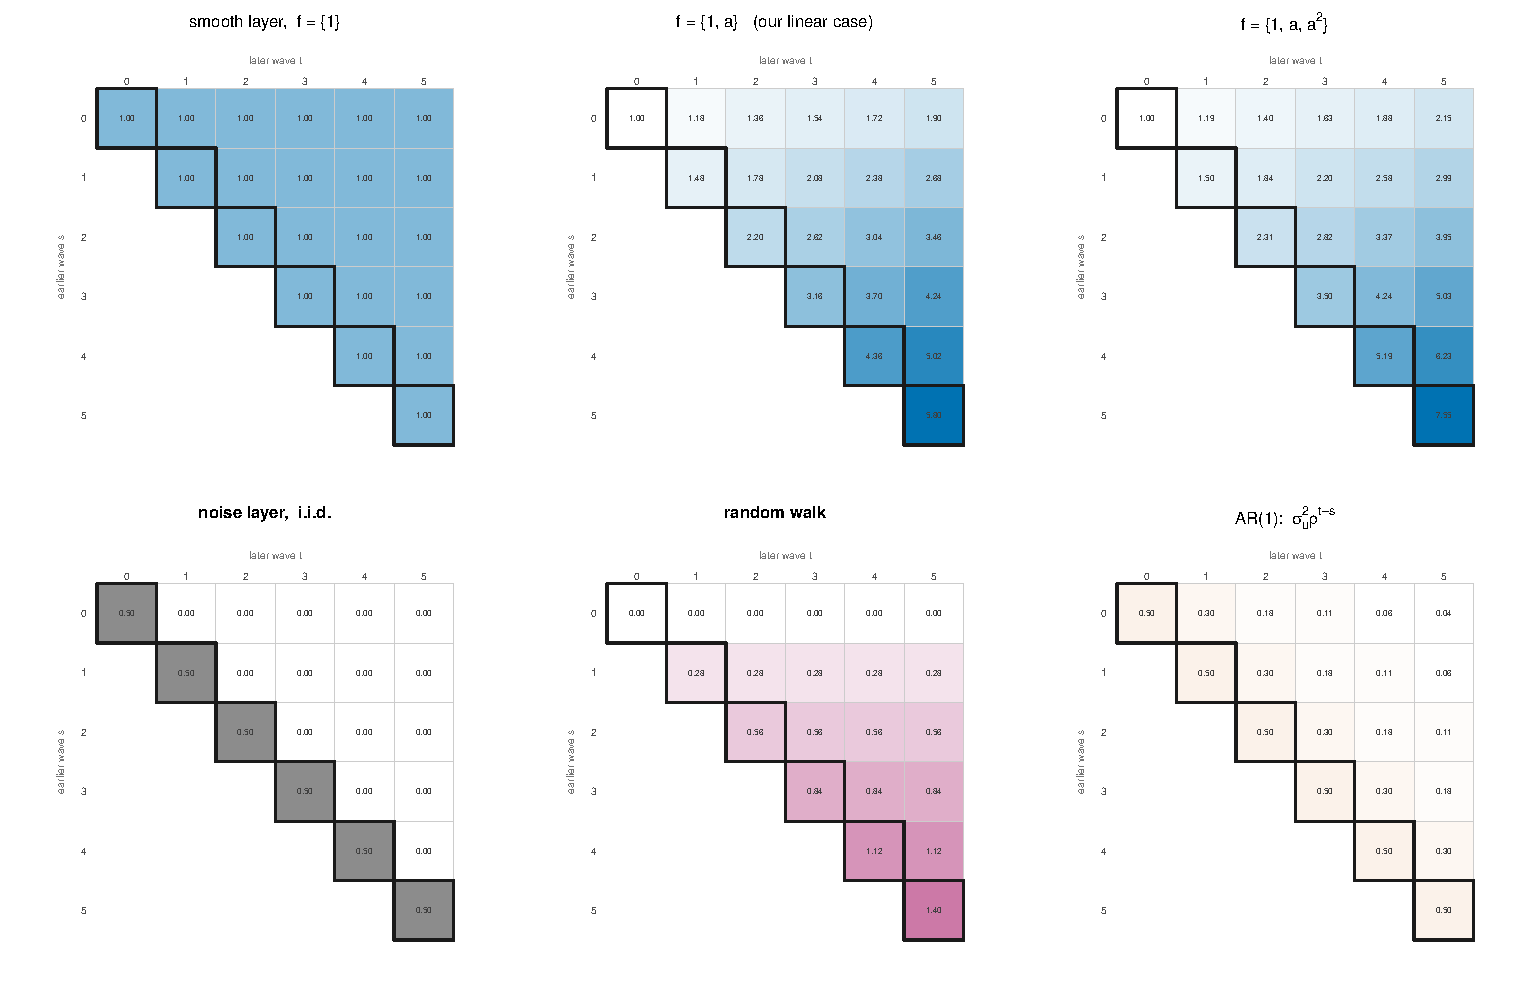
\includegraphics[width=\textwidth]{figures/fig_surface_menu_tri}
\end{figure}

\subsection*{Age-varying noise without memory: the denoising case}

Case 3 handles age-specific variances with memory. The memoryless version ($\rho=0$ with free $v_a$) is simpler and has its own device.

\emph{Independent noise, free $v_a$ (the denoising case).} Now no formula for $(V_H,C_{Hd},V_d)$ can put weight on any raw $\Var(h_a)$: each variance carries its own free $v_a$ that no other moment contains.
But off-diagonal cells are pure smooth layer, and because the smooth layer is linear along each row, the \emph{noise-free variance profile} can be rebuilt from them:
\begin{equation}
\Var^{*}(h_a)=\tfrac12\bigl[\Cov(h_{a-1},h_a)+\Cov(h_a,h_{a+1})\bigr]
\quad\text{(interior $a$; edges by extrapolation)},
\label{eq:varstar}
\end{equation}
after which everything is Case 1 run on the starred profile (Figure~\ref{fig:denoiseanat}): $v_a=\Var(h_a)-\Var^{*}(h_a)$, $V_d=\tfrac12[\Var^{*}(h_2)-2\Var^{*}(h_1)+\Var^{*}(h_0)]$, $C_{Hd}=\tfrac12[\Var^{*}(h_1)-\Var^{*}(h_0)-V_d]$, $V_H=\Var^{*}(h_0)$.
Three waves; algebraically identical to the covariance-only solve (Appendix~\ref{app:props}, the denoising case).

\begin{figure}[H]
	\caption{Illustration of the denoising case}
	\label{fig:denoiseanat}
	\centering
	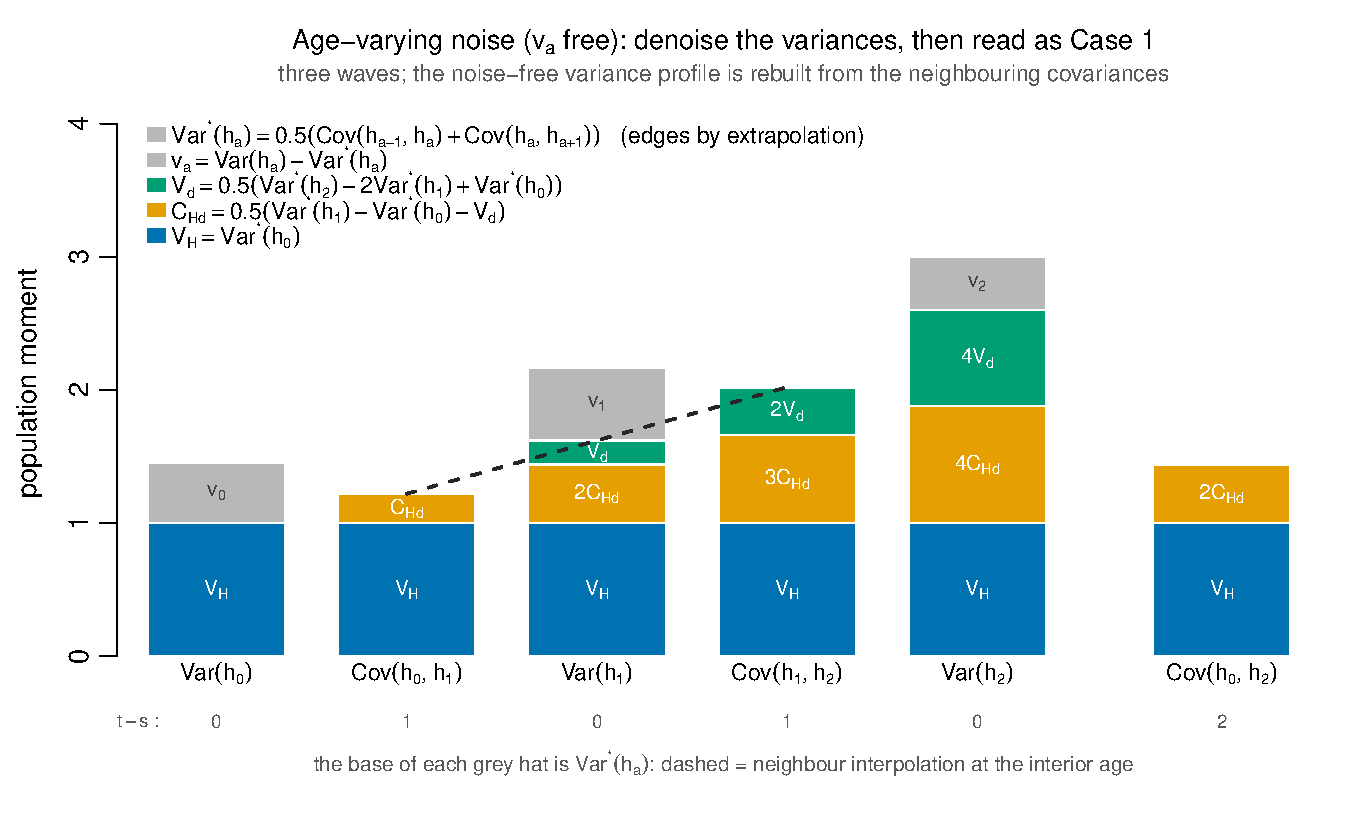
\includegraphics[width = 0.8 \linewidth]{figures/fig_denoise_anatomy}
\end{figure}

\emph{The general cases are Cases 3 and 4 in the main text.} Case 3's noise layer \eqref{eq:case3noise} nests the denoising case at $\rho=0$, Case 2 at constant $v_a$, and the random walk at $\rho=1$; adding Case 4's spike, the family also contains Proposition~\ref{prop:F1} below as its $\rho\to1$ member, so the main text's class now covers every noise model used in this note.
In practice we estimate that family plus a diagonal spike: minimum distance on \eqref{eq:template} with the layers \eqref{eq:case3noise} $+$ spike, with the main-text cases as the reading guide and the restrictions table below as the test menu.

\subsection*{The persistent-shocks case in full}

\begin{proposition}[Random walk plus measurement noise]\label{prop:F1}
Under A1-A2, let $u_{i,a}=w_{i,a}+\varepsilon_{i,a}$ with $w_{i,a}=w_{i,a-1}+\eta_{i,a}$, $\varepsilon$ i.i.d.\ over ages, all innovation variances free to vary with age, and shocks mutually uncorrelated.
The level covariances then satisfy, for $s<t$,
\begin{equation}
\Cov(h_s,h_t)\;=\;V_H+\Var(w_0)+(s+t)\,C_{Hd}+st\,V_d+\sum_{\ell=1}^{s}\sigma^2_{\eta,\ell}
\qquad\text{(the sum is empty for $s=0$)},
\end{equation}
so fixing the earlier wave $s$ and varying the later one leaves the noise terms untouched. With four waves:
\begin{align}
C_{Hd} &= \Cov(h_0,h_2)-\Cov(h_0,h_1) \quad\text{(off-diagonal read)},\\
V_d &= \bigl[\Cov(h_1,h_3)-\Cov(h_1,h_2)\bigr]-C_{Hd},\\
\sigma^2_{\eta,s} &= \bigl[\Cov(h_s,h_t)-\Cov(h_{s-1},h_t)\bigr]-C_{Hd}-t\,V_d \quad (\text{any } t>s),\\
\sigma^2_{\varepsilon,a} &= \Var(h_a)-\Cov(h_a,h_t)+(t-a)\bigl(C_{Hd}+a\,V_d\bigr) \quad (\text{any } t>a).
\end{align}
Levels identify $V_H$ only in the bundle $V_H+\Var(w_0)=2\Cov(h_0,h_1)-\Cov(h_0,h_2)$, but that doesn't matter for the returns to prevention/treatment.
\end{proposition}

\begin{itemize}
\item Reading: the staircase makes the noise variance non-stationary, so the variance profile is unusable here and every read is off-diagonal. Row $0$ keeps the denoising-case formulas because its noise sum is empty; moving along a row adds $C_{Hd}+rV_d$ per wave; crossing to the next row additionally picks up one permanent-shock variance; the diagonal sits $\sigma^2_{\varepsilon,a}$ above the off-diagonal formula (Figure~\ref{fig:F1anat}).
Distance from the diagonal never kills the staircase - direction does: row reads are staircase-immune.
\item Equivalent difference combinations: $\Cov(\Delta h_t,\Delta h_{t+k})=V_d$ and $\Cov(h_0,\Delta h_k)=C_{Hd}$ for $k\ge2$; at lag one, $\Cov(\Delta h_t,\Delta h_{t+1})=V_d-\sigma^2_{\varepsilon,t}$ (the mean-reversion dip).
\item $C_{Hd}$ needs 3 waves, $V_d$ needs 4. Everything else is identified except at the panel's edge (the last wave's $\sigma^2_\eta/\sigma^2_\varepsilon$ split is identified only in sum).
\end{itemize}

\begin{figure}[H]
	\caption{Illustration of Proposition~\ref{prop:F1}}
	\label{fig:F1anat}
	\centering
	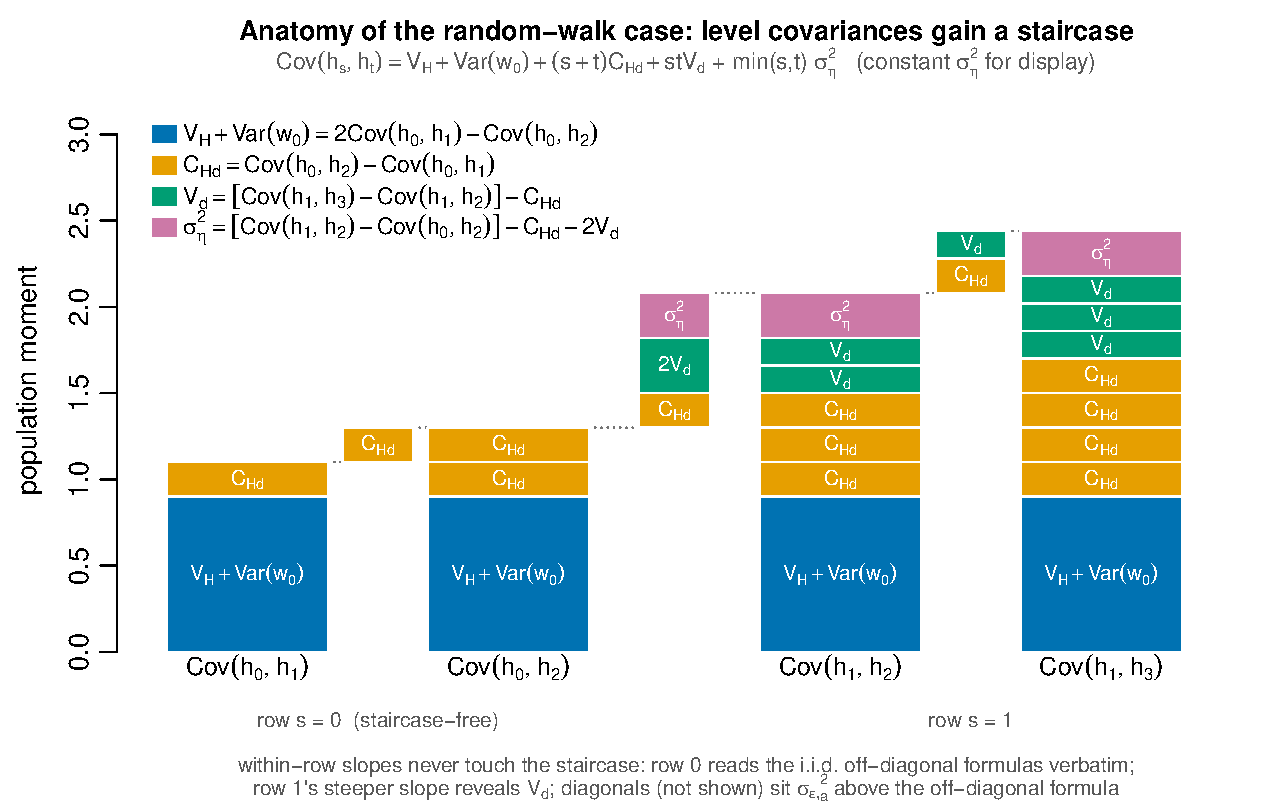
\includegraphics[width = 0.75 \linewidth]{figures/fig_prop3_anatomy_levels}
\end{figure}

\emph{Proof of Proposition~\ref{prop:F1}.} For $s<t$, $\Cov(u_s,u_t)=\Cov(w_s+\varepsilon_s,\,w_t+\varepsilon_t)=\Var(w_s) =\Var(w_0)+\sum_{\ell\le s}\sigma^2_{\eta,\ell}$ (the walk is shared up to the earlier wave; the $\varepsilon$'s share nothing), which added to \eqref{eq:forwardmap} gives the stated level covariances.
The reads follow by differencing: along a row, $t\mapsto t+1$ at fixed $s$ adds $C_{Hd}+rV_d$; across rows, $s\mapsto s+1$ at fixed $t$ adds $C_{Hd}+tV_d+\sigma^2_{\eta,s+1}$; and $\Var(h_a)-\Cov(h_a,h_t)=\sigma^2_{\varepsilon,a}-(t-a)(C_{Hd}+aV_d)$ gives the diagonal excess.
Row $0$ shows only the bundle: $\Cov(h_0,h_t)=\bigl(V_H+\Var(w_0)\bigr)+tC_{Hd}$.
For the difference combinations: $\Delta h_t=d+\eta_t+\varepsilon_t-\varepsilon_{t-1}$; for $k\ge2$ the noise terms share no common shock, so $\Cov(\Delta h_t,\Delta h_{t+k})=V_d$ and $\Cov(h_0,\Delta h_k)=C_{Hd}$; at $k=1$ the shared $\varepsilon_t$ contributes $-\sigma^2_{\varepsilon,t}$.
\qed

\subsection*{The cases as restrictions}

Each case is \eqref{eq:surface}/\eqref{eq:template} with layers switched off; each added layer costs waves; each switched-off layer is a testable restriction.

\begin{center}
\footnotesize
\begin{tabular}{@{}lllll@{}}
\toprule
& \textbf{Noise restriction} & \textbf{Fingerprint} & \textbf{Test} & \textbf{Waves} \\
\midrule
$C_{Hd}{=}0$ remark & i.i.d., stationary & flat row 0 & $C_0(1)=C_0(2)$ & 2 \\
Case 1 & i.i.d., stationary & quadratic diagonal & quadratic profile ($T{>}3$) & 3 \\
Case 2 & AR(1), stationary & geometric fade off-diagonal & constant fade ratio & 3 \\
denoising & independent, free $v_a$ & spike only & rows linear in $t$ & 3 \\
Case 3 & AR(1), free $v_a$ & fade $\times$ row amplitude & constant $S_k$ ratio & 4 \\
Case 4 & AR(1) $+$ spike & fade off-diagonal, ridge on & interior cells & 4 \\
Prop.~\ref{prop:F1} & random walk $+$ i.i.d. & staircase $+$ spike & flat $D_k$ from $k\ge2$ & 4 \\
\bottomrule
\end{tabular}

\smallskip
{\footnotesize Waves $=$ minimum for just-identification; running a row's test needs at least the next wave (the remark row's needs a third; the $D_k$ ladder a fifth).}
\end{center}

\subsection*{Limits}

\begin{itemize}
\item \emph{Two splits inside the equation.} $V_H$ vs.\ $\omega^2$: both live only in the level $B$ - for levels, a permanent stochastic position is a type intercept, which is the framework's own message and the $\rho\to1$ limit of Section~\ref{sec:forces} (neither part is needed for the returns).
And at the panel's edge, $G(T-1)$ appears only in the last diagonal cell, so the final wave's split is identified only in sum.
\item \emph{Persistence outside the class.} A $\gamma_u$ outside the family \eqref{eq:case3noise} - for example Case 3 plus an i.i.d.\ spike, or MA($q$) components - loses the clean reads.
Identification is then by minimum distance on \eqref{eq:template}.
A rising lag-$\ge2$ ladder $D_k$ under the fitted class is the sign that the class is too small.
\item \emph{Distributional shape.} The surface sees only second moments of $(H_i,d_i)$; the number and location of types, multimodality, and tail behaviour are invisible - clustering's job, and exactly what the targeting appendix needs (Appendix~\ref{sec:targeting}).
\item \emph{Selection.} With health-related attrition or mortality the observed surface is conditional on survival, and the single-equation story needs reweighting or an explicit survival margin.
Flagged, not solved.
\end{itemize}



%% =============================================================================
\section{A first empirical pass at the local covariance (parked)}\label{app:localpass}
%% =============================================================================

This appendix records a first attempt at estimating the local level-change covariance $C_{Hd}(a)$ of Section~\ref{sec:back} from the UKHLS covariance rows, so that the results can be picked up again when the full empirical section is built.
The main text deliberately stops at illustration; nothing before this appendix uses these estimates.
The estimator library and its simulation gates (\texttt{emp\_26\_row\_estimator\_fns.R}, \texttt{emp\_26\_local\_rows.R}, \texttt{check\_row\_estimator.R}) live with the empirical companion repo.

\subsection*{What was estimated}

\begin{itemize}
\item For each base age $s$, the row $\Cov(h_s,h_{s+k})$, $k=0,\dots,9$, was fitted per anchor; the slope of the deterministic part is $C_{Hd}(s)$.
\item The fits differ only in how the noise is treated, and each was gated on simulated data before touching the data.
\item Over a nine-year row a slow fade, a curve and a straight line partially mimic one another, so no single treatment is unbiased under every noise process; a suite is used and its spread is reported as model uncertainty.
\item The suite: a \emph{bundle} fit (one-year spike $+$ quadratic, no decay column; exact when the persistent noise is near-permanent - the corner the data itself selects, and the $\rho\to1$ bundle limit of Section~\ref{sec:forces}); a per-anchor quadratic-plus-decay fit (exact under pure AR(1) noise; biased late under spike mixtures); a line-plus-decay fit (reads the row-average local covariance; the early side of the bracket); the four-cell just-identified read of \eqref{eq:rowreads3}; and a common-$\rho$ joint fit (recorded, but degenerate here: the data pushes $\rho$ to the top of the grid, where the decay column is collinear with the line).
\item Person-level bootstrap (300 replicates) supplies the confidence bands; row lengths $K=6,9,12$ as sensitivity.
\end{itemize}

\subsection*{What the data said}

\begin{itemize}
\item On the primary measure, $C_{Hd}(a)$ sits at or just below zero through ages 20-50 and turns decisively negative from the late 50s, reaching $-0.002$ to $-0.004$ per year by 70-80 (Figure~\ref{fig:localCHd}).
\item The same shape appears under every treatment in the suite and on every measure (Figure~\ref{fig:localCHdall}); the flattest is the SF-6D, as elsewhere.
\item A single ``crossing age'' is not a robust object: the young-age sign straddles zero, so the formal zero-crossing moves between about 55 and 71 with the noise treatment. The robust statements are the break and the late-life magnitude.
\item The noise anatomy is a finding in itself: a large one-year spike plus a near-permanent slow layer. Profiling the fade speed runs to the top of the grid - the bundle limit of Section~\ref{sec:forces} operating in the data - which is why the bundle fit is the primary.
This structure is Case 4 of Section~\ref{sec:cases} at its $\rho\to1$ corner: what Case 4 identifies cleanly with a fourth wave when $\rho$ is away from one, the suite here handles at the corner by folding the carried part into the level.
\item The spike \emph{level} rises with age (roughly $0.005$ to $0.009$ on the primary measure over ages 20-80); it is the spike's \emph{share} of the variance that falls.
\item Corroboration from changes: the $D_k$ plateau by age band is most negative at ages 60-70 on the PCS measures - the change-based signature of the same compression.
\end{itemize}

\subsection*{Caveats carried forward}

\begin{itemize}
\item Every row conditions on being observed $k$ years later, so these are survivors' covariances; the selection, floor and cohort-pooling treatments belong to the empirical section and have not been applied here.
\item With the young-age covariance at zero rather than positive, compounding is weak at best on these measures; the strong empirical fact is the compression after 60.
\end{itemize}

\begin{figure}[H]
	\caption{The local covariance $C_{Hd}(a)$ on the primary measure: bundle fit with 95\% bootstrap band, and the spike level by age.}
	\label{fig:localCHd}
	\centering
	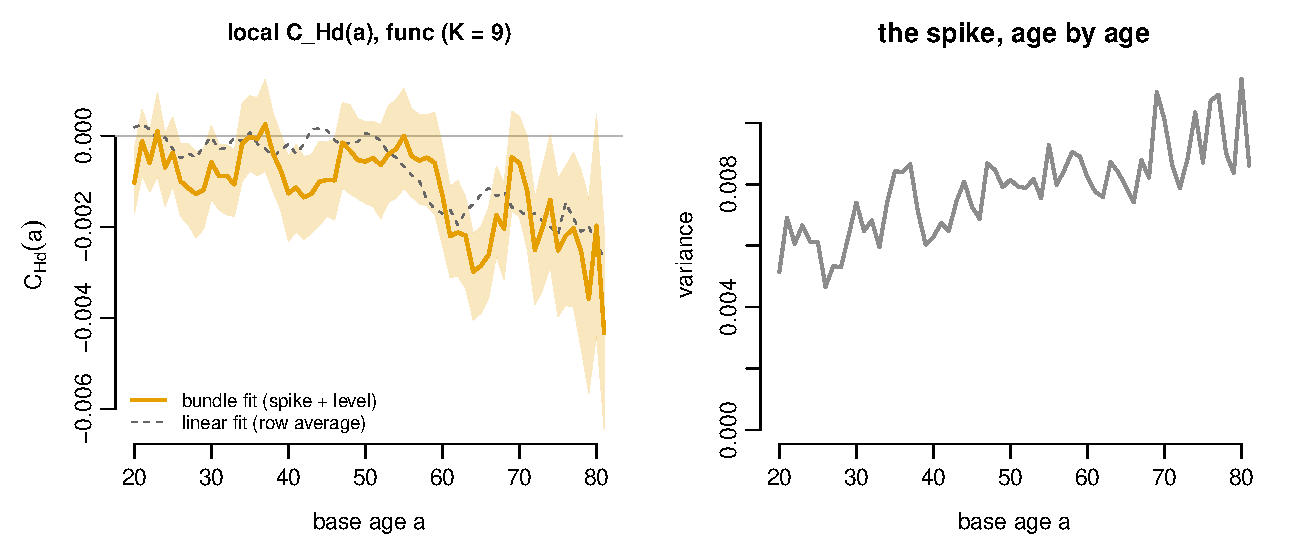
\includegraphics[width=0.9\linewidth]{emp_fig_localCHd}
\end{figure}

\begin{figure}[H]
	\caption{The same profile across the six measures ($K=9$).}
	\label{fig:localCHdall}
	\centering
	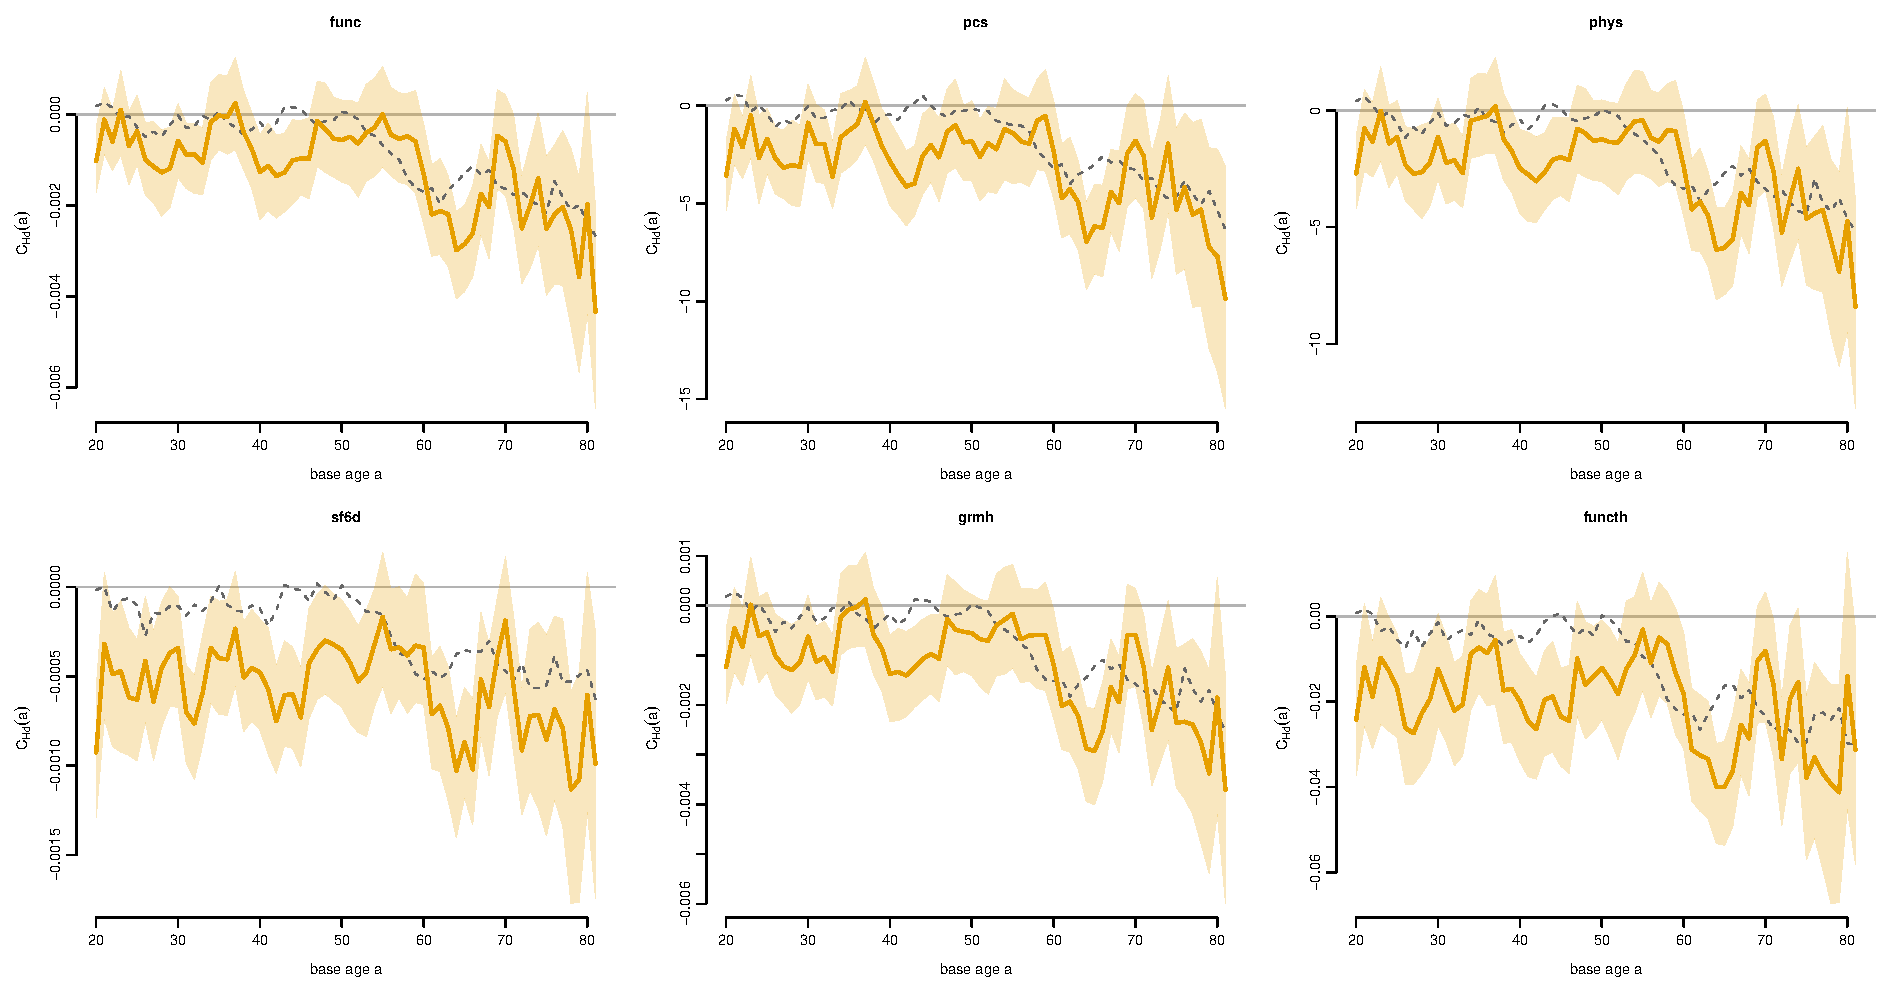
\includegraphics[width=\linewidth]{emp_fig_localCHd_all}
\end{figure}

\end{document}
